%%%%%%%%%%%%%%%%%%%%%%%%%%%%%%%%%%%%%%%%%%%%%%%%%%%%%%%%%%%%%%%%%%%%%%%%
\chapter{L'\ensemble\ canonico}
\label{cap:canonico}
%%%%%%%%%%%%%%%%%%%%%%%%%%%%%%%%%%%%%%%%%%%%%%%%%%%%%%%%%%%%%%%%%%%%%%%%

Per molte ottime ragioni considerare esattamente fissata l'energia di un sistema fisico non è una buona idea. {\em In primis} occorre notare che una misura diretta ed esatta dell'energia interna di un sistema termodinamico è a tutti gli effetti pratici impossibile (in genere l'energia è ricavata indirettamente, da misure di altre osservabili fisiche). In secondo luogo sappiamo bene che misurando un'osservabile qualsiasi di un sistema fisico perturbiamo il sistema stesso. \`E vero che almeno classicamente possiamo pensare di rendere trascurabile la perturbazione dovuta alla misura ma è anche vero che in ultima analisi stiamo considerando la fisica dei costituenti elementari di un corpo macroscopico: come abbiamo già avuto occasione di notare, tali costituenti elementari obbediranno alle leggi quantistiche. Poco male, diranno subito i miei piccoli lettori: possiamo, come abbiamo già fatto, assumere che l'energia fluttui intorno al valore $E$ di una quantità $\Delta$. La risposta a questa obiezione è duplice: da una parte, la fluttuazione $\Delta$ è (quasi) completamente arbitraria, e la sua comparsa nei calcoli dovrebbe essere evitata; dall'altra, $\Delta$ non può essere completamente arbitrario, come abbiamo visto; in particolare non può andare a $0$ nel limite termodinamico, pena la comparsa di divergenze in quantità fisiche. Solo il rapporto $\Delta/E$ deve andare a zero. (Di fatto che la meccanica statistica {\em classica} funzioni è alla fin fine solo un miracolo d'equilibrismo).

Possiamo pensare di tenere costante qualcos'altro, al posto dell'energia? La risposta è ovviamente sì. La relazione tra temperatura ed energia delle molecole di un gas ideale, nella teoria cinetica, ci suggerisce che potremmo tenere costante la temperatura $T$ e lasciare che l'energia possa liberamente fluttuare. In pratica consideriamo macrostati che non sono più caratterizzati dalla terna $(N\,,\,V\,,E)$ ma dalla terna $(N\,,\,V\,,T)$. Come vedremo  presto, la sorprendente risposta a questa richiesta è che di fatto non cambia niente.

%%%%%%%%%%%%%%%%%%%%%%%%%%%%%%%%%%%%%%%%%%%%%%%%%%%%%%%%%%%%%%%%%%%%%%%%
\section{Sistema all'equilibrio con una riserva termica}
%%%%%%%%%%%%%%%%%%%%%%%%%%%%%%%%%%%%%%%%%%%%%%%%%%%%%%%%%%%%%%%%%%%%%%%%

Immaginiamo che il nostro sistema fisico sia in contatto termico con una riserva, ossia un sistema molto più grande (al limite, l'intero Universo). L'energia del sistema totale è conservata, e sarà uguale alla somma delle energie dei due sistemi:
\be
E_0 = E_r + E'_r
\ee
in cui $E_r$ è l'energia del nostro sistema fisico ed $E'_r$ l'energia della riserva termica. Notiamo che i due sistemi, essendo in contatto termico e all'equilibrio, avranno una temperatura comune, $T$, ma in ogni caso l'energia di ciascuno potrà variare tra $0$ e $E_0$, fermo restando il fatto che la loro somma deve rimanere costante. La riserva termica serve a garantire che il sistema fisico che stiamo considerando resti a temperatura costante $T$. Ora, poiché la riserva termica è molto più grande del nostro sistema, possiamo tranquillamente chiedere che in ogni istante di tempo debba valere
\be
\label{eq:cond1}
E_r \ll E'_r
\ee
e quindi $E'_r$ sarà sempre molto vicina a $E_0$; a tutti gli effetti pratici possiamo considerare la riserva come un sistema con un'energia fissata, e trattarla quindi con i metodi microcanonici.
Chiamiamo $\Omega'(E'_r)$ il numero dei microstati della riserva termica compatibili con l'energia $E'_r$; risulterà chiaro che più grande $\Omega'(E'_r)$, più grande la probabilità che il sistema fisico abbia energia $E_r$. Se inoltre si considera che tutti i microstati compatibili con $E'_r$ sono ugualmente probabili si arriva alla conclusione che la probabilità $P_r$ di osservare un'energia $E_r$ nel sistema fisico è direttamente proporzionale a $\Omega'(E'_r)$ stesso.

Tenendo conto della (\ref{eq:cond1}) possiamo espandere intorno al caso $E_r \simeq 0$:
\be
\ln\Omega'(E'_r) = \ln\Omega'(E_0) + E_r\dpar{\ln\Omega'}{E'_r} + \cdots \simeq \mbox{\textrm{cost}} - \beta'E_r
\ee
e ricordando che all'equilibrio $\beta' = \beta \equiv 1/kT$ otteniamo subito
\be
P_r \propto e^{-\beta E_r}
\ee
Per normalizzare richiediamo che la probabilità totale sia uguale a $1$, e abbiamo quindi
\be
P_r = \frac{e^{-\beta E_r}}{\sum_s e^{-\beta E_s}}
\ee

%%%%%%%%%%%%%%%%%%%%%%%%%%%%%%%%%%%%%%%%%%%%%%%%%%%%%%%%%%%%%%%%%%%%%%%%
\section{L'\ensemble\ canonico}
%%%%%%%%%%%%%%%%%%%%%%%%%%%%%%%%%%%%%%%%%%%%%%%%%%%%%%%%%%%%%%%%%%%%%%%%

Consideriamo un \ensemble\ di $\calN$ copie mentali dello stesso sistema fisico; $n_k$ rappresenta il numero di copie con energia $E_k$. L'energia totale dell'\ensemble, ossia la somma di tutte le energie dei sistemi nell'\ensemble, vale $\calE$. Naturalmente $E_k$ e $n_k$ devono soddisfare i vincoli
\bea
\label{eq:condcan}
\sum_{k}n_k      &=& \calN\nonumber\\
\sum_{k} E_k n_k &=& \calE \equiv U\calN
\eea
in cui $U$ è l'energia media dell'\ensemble\ che coincide proprio con l'energia interna del sistema fisico originale. 
Qualsiasi insieme $\nkset$ che soddisfi i vincoli (\ref{eq:condcan}) rappresenta un modo possibile di distribuire l'energia $\calE$ tra gli $\calN$ membri dell'\ensemble. Inoltre ognuno di questi modi possibili può essere ottenuto in molti modi diversi, perché possiamo sempre pensare di permutare i sistemi: per esempio potremmo prendere un sistema con energia $E_1$ e scambiarlo con un sistema con energia $E_5$, ottenendo un altro modo possibile di avere lo stesso set $\nkset$. Chiamiamo $\Wnk$ il numero di modi in cui possiamo ottenere il set $\nkset$:
\be
\label{eq:W}
\Wnk = \frac{\calN!}{n_0!n_1!n_2!\cdots}
\ee
Considerando che tutti i possibili stati dell'\ensemble\ compatibili con le (\ref{eq:condcan}) hanno la stessa probabilità di occorrere, la frequenza con cui apparirà un determinato insieme 
$\nkset$ sarà proporzionale a $\Wnk$

Il nostro obiettivo è quello di calcolare la probabilità $P_k$ di trovare uno degli elementi dell'\ensemble\ in uno stato con energia $E_k$; naturalmente avremo
\be
P_k = \frac{\aspetta{n_k}}{\calN}
\ee
in cui per definizione di media sull'\ensemble\ avremo
\be
\label{eq:nrmean}
\aspetta{n_k} = \frac{\sum_{\nkset}'n_k \Wnk}{\sum_{\nkset}' \Wnk}
\ee
e l'apice sulle sommatorie serve a ricordare che le sommatorie stesse devono essere fatte rispettando i vincoli (\ref{eq:condcan}). Possiamo anche cercare l'insieme $\nkset$ più probabile, $n_k^*$; come vedremo, nel limite $\calN\to\infty$ i due risultati coincidono. Cominciamo quindi la derivazione dell'\ensemble\ canonico con il metodo del valore più probabile.

%%%%%%%%%%%%%%%%%%%%%%%%%%%%%%%%%%%%%%%%%%%%%%%%%%%%%%%%%%%%%%%%%%%%%%%%
\subsection{Il metodo del valore più probabile}
%%%%%%%%%%%%%%%%%%%%%%%%%%%%%%%%%%%%%%%%%%%%%%%%%%%%%%%%%%%%%%%%%%%%%%%%

L'insieme $n_k^*$ sarà tale da massimizzare $\Wnk$. Come al solito lavoriamo con il logaritmo e assumiamo che $n_k\gg 1$ per ogni $k$:
\be
\label{eq:lnW}
\ln W = \ln(\calN!) - \sum_k\ln(n_k!) \simeq \calN\ln\calN - \sum_k n_k\ln n_k
\ee
in cui nell'ultimo passaggio abbiamo usato la formula di Stirling. Se adesso passiamo da $\nkset$ a un insieme leggermente diverso, $\dnkset$, l'espressione (\ref{eq:lnW}) cambierà di una quantità
\be
\delta(\ln W) = -\sum_k(\ln n_k + 1)\delta n_k
\ee
e se il set $\nkset$ è quello più probabile allora $\delta(\ln W) = 0$. A causa dei vincoli (\ref{eq:condcan}) le variazioni $\delta n_k$ non possono essere arbitrarie, ma devono a loro volta sottostare ai vincoli
\bea
\sum_k \delta n_k     &=& 0\nonumber\\
\sum_k E_k \delta n_k &=& 0
\eea
Il set $n_k^*$ viene quindi calcolato usando il metodo dei moltiplicatori di Lagrange; la condizione che determina $n_k^*$ è
\be
\sum_k[-(\ln n_k^* + 1) - \alpha - \beta E_k]\delta n_k = 0
\ee
Grazie ai moltiplicatori le variazioni $\delta n_k$ sono diventate indipendenti e completamente arbitrarie; perché la somma sia nulla devono quindi essere nulli tutti i coefficienti:
\be
\ln n_k^* = -(\alpha+1) - \beta E_k
\ee
e cioè
\be
n_k^* = C\exp(-\beta E_k)
\ee
in cui $\alpha$ è stato riassorbito nella costante di normalizzazione $C$.
Poiché interpretiamo $n_k^*/\calN$ come la probabilità di trovare un elemento dell'\ensemble\  con energia $E_k$, $C$ scompare con l'ovvia normalizzazione
\be
\frac{n_k^*}{\calN} = \frac{\exp(-\beta E_k)}{\sum_r\exp(-\beta E_r)}
\ee
mentre il parametro $\beta$ è la soluzione dell'equazione
\be
\frac{\calE}{\calN} = U = \frac{\sum_k E_k\exp(-\beta E_k)}{\sum_k \exp(-\beta E_k)}
\ee
Come vedremo in seguito, è naturale identificare ancora una volta $\beta$ con l'inverso di $kT$.

%%%%%%%%%%%%%%%%%%%%%%%%%%%%%%%%%%%%%%%%%%%%%%%%%%%%%%%%%%%%%%%%%%%%%%%%
\subsection{Il metodo di Darwin--Fowler}
%%%%%%%%%%%%%%%%%%%%%%%%%%%%%%%%%%%%%%%%%%%%%%%%%%%%%%%%%%%%%%%%%%%%%%%%

Il nostro obiettivo è ora quello di calcolare $\aspetta{n_k}$; vedi eq. (\ref{eq:nrmean}). Per prima cosa introduciamo dei parametri reali $w_k$ e definiamo la funzione
\be
\widetilde{W}\nkset = \Wnk w_0^{n_0} w_1^{n_1} w_2^{n_2}\dots 
\ee
Introduciamo ora
\be
\label{eq:gamnu}
\Gamma(\calN,U) \equiv \sum_{\nkset}''\widetilde{W}\nkset
\ee
dove si nota che la sommatoria è ancora sottoposta ai vincoli (\ref{eq:condcan}). Il motivo per cui si è scelto di indicare i vincoli con due apici sarà chiaro tra poco. La definizione (\ref{eq:gamnu}) ci permette di scrivere
\be
\aspetta{n_k} = w_k\dpar{}{w_k}\ln\Gamma(\calN,U)|_{w_r = 1\;\;\forall\;\;r}
\ee
Dalla definizione di $\widetilde{W}\nkset$ abbiamo subito che
\be
\label{eq:gamnu2}
\Gamma(\calN,U) \equiv \sum_{\nkset}''\calN!\frac{w_0^{n_0}}{n_0!}
\frac{w_1^{n_1}}{n_1!}\frac{w_2^{n_2}}{n_2!}\cdots
\ee
Ora, se non ci fosse il secondo dei vincoli (\ref{eq:condcan}) ma solo il primo, potremmo calcolare $\Gamma(\calN,U)$ al volo, applicando banalmente il teorema multinomiale (vedi sezione (\ref{subsec:app1-multinomiale}) dell'Appendice \ref{app:matematica}):
\be
\Gamma(\calN,U) = (w_0 + w_1 + w_2 + \cdots)^\calN
\ee
Per poter ricavare $\Gamma$ introduciamo un'altra funzione:
\bea
\label{eq:gammatilde}
\widetilde{\Gamma}(\calN,U;z) &\equiv& \sum_{\nkset}'\calN!\frac{w_0^{n_0}}{n_0!}
\frac{w_1^{n_1}}{n_1!}\frac{w_2^{n_2}}{n_2!}\cdots z^\calE\nonumber\\
&=& \sum_{\nkset}'\calN!\frac{w_0^{n_0}}{n_0!}
\frac{w_1^{n_1}}{n_1!}\frac{w_2^{n_2}}{n_2!}\cdots z^{n_0E_0 + n_1E_1 + n_2E_2 + \cdots}\nonumber\\
&=& \sum_{\nkset}'\calN!\frac{(w_0 z^{E_0})^{n_0}}{n_0!}
\frac{(w_1 z^{E_1})^{n_1}}{n_1!}\frac{(w_2 z^{E_2})^{n_2}}{n_2!}\cdots
\eea
in cui $z$ è una variabile complessa. Ora l'apice sulla sommatoria è diventato solo uno, per ricordarci che il secondo dei vincoli, quello sull'energia, è caduto: il vincolo sull'energia è stato implementato quando abbiamo scritto esplicitamente, nella (\ref{eq:gammatilde}), $z^\calE = z^{n_0E_0+n_1E_1+...}$. Rimane dunque solo il primo vincolo.

A questo punto dobbiamo ricorrere a un trucco. Prima di tutto, poiché l'energia, almeno classicamente, è sempre definita a meno di una costante additiva arbitraria, siamo liberi di porre $E_0 = 0$. Inoltre scegliamo un'unità di misura per l'energia talmente fine da rendere le $E_k$ numeri interi a tutti gli effetti pratici (se si pensa ai livelli di energia quantistici di una particella in una scatola si vede subito che questo è certamente possibile). Inoltre la nostra unità di misura per l'energia è tale che le $E_k$ non hanno nessun divisore comune (questa è un'assunzione che ci servirà in seguito). Per giustificare la fondatezza di quest'ultima assunzione basti pensare che se gli $E_k$ avessero un divisore comune allora anche $\calE$ l'avrebbe, perché altrimenti il secondo dei vincoli (\ref{eq:condcan}) non sarebbe soddisfatto. Sia ora $\tau$ il massimo comun divisore: in altre parole posso sempre scrivere
\be
\tau\calE' = \tau\sum_k n_k E_k'
\ee
in cui le variabili primate continuano a essere numeri interi. Se ora divido entrambi i membri per $\tau$ ottengo energie con valori interi senza nessun divisore comune (globale).

Adesso possiamo finalmente applicare il teorema multinomiale e scrivere
\be
\label{eq:serie1}
\widetilde{\Gamma}(\calN,U;z) = (w_0 z^{E_0} + w_1 z^{E_1} + w_2 z^{E_2} + \cdots)^\calN \equiv f^\calN(z)
\ee
Ora espandiamo in serie la funzione, scrivendo
\be
\label{eq:serie2}
\widetilde{\Gamma}(\calN,U;z) = \sum_n\Gamma_n z^n
\ee
e risulta subito evidente dalla definizione (\ref{eq:gammatilde}) che $\Gamma(\calN,U) = \Gamma_{\calE}$ (ricordiamo che $\calE$, con la nuova scala dell'energia, è diventato un numero intero). Per il nostro calcolo dobbiamo quindi solo ricavare il coefficiente $\Gamma_{\calE}$ dell'espansione, e il teorema dei residui ci permette di scrivere
\be
\label{eq:residui}
\Gamma(\calN,U) = \frac{1}{2\pi i}\oint\frac{\widetilde{\Gamma}(\calN,U;z)}{z^{\calE+1}}\de z
\ee
La serie (\ref{eq:serie2}) ha un raggio di convergenza $\rho$ (quale che sia, $\rho \le 1$). Se si analizza separatamente il comportamento del numeratore e del denominatore della funzione integranda nella (\ref{eq:residui}) (vedi figura \ref{fig:x0}) ci si rende subito conto che la funzione integranda stessa deve avere, sull'asse reale, un unico minimo per un valore $x_0 < 1$ della parte reale $x$ di $z = x + iy$. Intuitivamente possiamo ragionare così; nella funzione integranda il numeratore parte da $1$ per $z=0$ e va monotonicamente all'infinito positivo verso il bordo di convergenza della serie (\ref{eq:serie1}). Il fattore $z^{-\calE-1}$ parte dall'infinito positivo per $z=0$ e decresce monotonicamente verso $0$, conservando un valore finito sul bordo di convergenza della serie (\ref{eq:serie1}). Che ci debba essere un minimo in $x_0$, con $0 < x_0 < 1$ è evidente. Per i dettagli della dimostrazione che il minimo è unico si veda \cite{Schr}.
%%%%%%%%%%%%%%%%%%%%%%%%%%%%%%%%%%%%%%%%%%%%%%%%%%%%%%%%%%%%%%%%%%%%%%%%%
\begin{figure}[h]
  \centering
  \begin{tikzpicture}[scale=10]
  \draw[->] (-0.05,0) -- (1.1,0);
  \draw[->] (0,-0.05) -- (0,1);
  \draw[color=red!80!black]  (0.005,0.9) .. controls (0.1,0.1) and (0.5,0.01) .. (0.9,0.005);
  \draw[color=blue!80!black] (0,0.1)     .. controls (0.8,0.2) and (0.99,0.5) .. (0.995,1);
  \draw (0.03,0.8) .. controls (0.2,0.2) and (0.92,0.2) .. (0.98,0.9);
  
  \draw[dotted] (1,0) -- (1,1);
  \draw (1,-0.03) node{$\rho$};
  \draw[dotted] (0.52,0) -- (0.52,0.36);
  \draw (0.52,-0.03) node{$x_0$};
  
  \draw[color=red!80!black] (0.7,0.05) node{$x^{-\mathcal{E}-1}$};
  \draw[color=blue!80!black] (0.7,0.25) node{$f^{\mathcal{N}}(x)$};
\end{tikzpicture}

  \caption{Determinazione di $x_0$} 
  \label{fig:x0}
\end{figure}
%%%%%%%%%%%%%%%%%%%%%%%%%%%%%%%%%%%%%%%%%%%%%%%%%%%%%%%%%%%%%%%%%%%%%%%%%
Per ottenere la condizione di minimo scriviamo
\be
\frac{f^\calN(z)}{z^{\calE+1}} \equiv e^{\calN g(z)}
\ee
e poiché il circuito chiuso nell'integrale della (\ref{eq:residui}) è arbitrario, lo prendiamo essere un cerchio di raggio $x_0$. La condizione di minimo
\be
\frac{\de e^{\calN g(x)}}{\de x} = 0
\ee
diventa subito
\be
\frac{\de g(x)}{\de x} = 0
\ee
con
\be
g(x) = \frac{1}{\calN}(\calN\ln f - (\calN U + 1)\ln x) \simeq \ln f - U\ln x
\ee
in cui nell'ultimo passaggio abbiamo sfruttato il fatto che $\calN U \gg 1$. Abbiamo dunque la condizione
\be
\label{eq:condmin}
g'(x_0) = \frac{f'(x_0)}{f(x_0)} - \frac{U}{x_0} = 0
\ee
Teniamo a mente questo risultato: anche nel limite $\calN\to\infty$, il valore di $x_0$ è indipendente da $\calN$. Poi, ricordando che
\be
f(x) = \sum_k w_k x^{E_k}
\ee
otteniamo subito
\be
x_0 f'(x_0) = \sum_k E_k w_k x_0^{E_k}
\ee
e introducendo il parametro $\beta$
\be
x_0 \equiv e^{-\beta}
\ee
dalla (\ref{eq:condmin}) possiamo ricavare immediatamente
\be
U = \frac{\sum_k E_k w_k e^{-\beta E_k}}{\sum_k w_k e^{-\beta E_k}}
\ee
\`E da notare che come nel caso del valore più probabile, anche qui $\beta$ lo si ricava dall'equazione precedente, una volta che tutte le $w_k$ siano state poste uguali a 1, come occorre fare alla fine del procedimento.
Dobbiamo ora considerare cosa succede se, partendo da $x_0$, ci spostiamo lungo la direzione immaginaria $y$. Le relazioni di Cauchy--Riemann,
\be
\frac{\partial^2 f}{\partial x^2} = -\frac{\partial^2 f}{\partial y^2}
\ee
ci dicono che se in $x_0$ in direzione $x$ c'è un minimo molto profondo, nello stesso punto, in direzione $y$, ci sarà un massimo estremamente pronunciato. In altre parole $x_0$ è un {\em punto di sella} (vedi figura \ref{fig:sella}; per un esempio pratico di punto di sella si pensi appunto a una sella o a una patatina {\em Pringles}). Calcoliamo la derivata seconda di $g(x)$ nel punto $x_0$:
\bea
g''(x_0) &=& \frac{f''(x_0)}{f(x_0)} - \left(\frac{f'(x_0)}{f(x_0)}\right)^2 + \frac{U}{x_0^2}\nonumber\\
&=& \frac{f''(x_0)}{f(x_0)} - \frac{U^2-U}{x_0^2}
\eea
%%%%%%%%%%%%%%%%%%%%%%%%%%%%%%%%%%%%%%%%%%%%%%%%%%%%%%%%%%%%%%%%%%%%%%%%%
\begin{figure}[h]
  \centering
  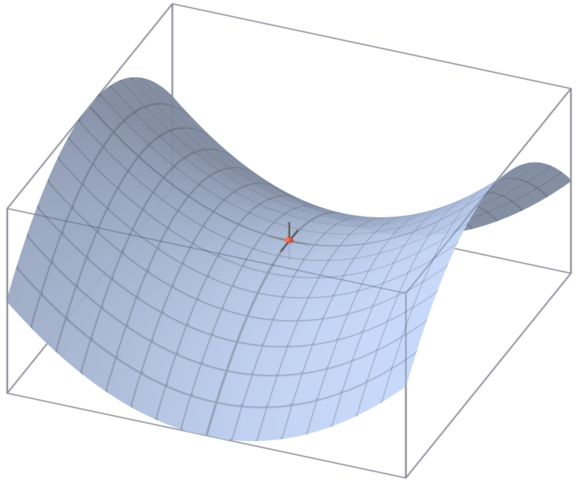
\includegraphics[width=0.7\textwidth]{saddle-point.png}
  \caption{Un punto di sella} 
  \label{fig:sella}
\end{figure}
%%%%%%%%%%%%%%%%%%%%%%%%%%%%%%%%%%%%%%%%%%%%%%%%%%%%%%%%%%%%%%%%%%%%%%%%%
Notiamo che anche $g''(x_0)$ rimane indipendente da $\calN$ nel limite $\calN\to\infty$. Per svolgere l'integrale (\ref{eq:residui}) ragioniamo in questo modo: tenendo conto che nel limite $\calN\to\infty$ il minimo in direzione $x$ è {\em molto profondo} e il massimo in direzione $y$ è {\em molto piccato}, spezziamo l'integrale circolare in due parti: un breve tratto (da $-\varepsilon$ a $\varepsilon$), che possiamo considerare rettilineo, in direzione immaginaria; e poi il resto della circonferenza:
\be
\label{eq:spezza}
\frac{1}{2\pi i}\oint \frac{f^\calN}{z^{\calE+1}}\de z =
\frac{1}{2\pi i}\left\{ \int_{-\varepsilon}^{\varepsilon}\frac{f^\calN}{y^{\calE+1}} i \de y
+\int_{C}\frac{f^\calN}{z^{\calE+1}}\de z\right\}
\ee
in cui la curva $C$ nel secondo integrale a destra è quasi tutta la circonferenza tranne il pezzettino di lunghezza $2\varepsilon$ che abbiamo spostato nell'integrale in $\de y$. Come vedremo in seguito, nel limite $\calN\to\infty$ l'integrale su $C$ nella (\ref{eq:spezza}) diventa trascurabile; per il momento lo ignoriamo. Per quel che riguarda invece il primo integrale, considerando che solo la regione immediatamente vicina a $x_0$ dà contributi significativi, siamo liberi di mandare $\varepsilon\to\infty$. Se approssimiamo $g(z)$, in direzione $y$, con il suo sviluppo in serie di Taylor al secondo ordine,
\be
g(z) \simeq g(x_0) - \frac{1}{2}y^2g''(x_0)\quad\mbox{\textrm{in direzione}}\ y
\ee
otteniamo immediatamente
\be
\label{eq:gammanu}
\Gamma(\calN,U) \simeq \frac{1}{2\pi}\frac{f^\calN(x_0)}{x_0^{\calE+1}}\int_{-\infty}^{\infty}\de y\; e^{-\calN a y^2/2} = \frac{f^\calN(x_0)}{x_0^{\calE+1}\sqrt{2\pi\calN a}}
\ee
in cui abbiamo posto $g''(x_0)\equiv a$. Possiamo quindi scrivere
\be
\frac{1}{\calN}\ln\Gamma(\calN,U) = \ln f(x_0) - \frac{\calE+1}{\calN}\ln x_0 - \frac{1}{2\calN}\ln(2\pi\calN a)
\ee
Notiamo due cose: prima di tutto possiamo porre $(\calE+1)/\calN\simeq U$, perché $\calE\gg 1$; in secondo luogo vediamo che l'ultimo termine scompare nel limite $\calN\to\infty$ in virtù del fatto che $a$ è indipendente da $\calN$. Otteniamo quindi
\be
\label{eq:lgamma}
\frac{1}{\calN}\ln\Gamma(\calN,U) = \ln\left(\sum_k w_k e^{-\beta E_k}\right) + \beta U
\ee
Finalmente possiamo scrivere
\bea
\frac{\aspetta{n_r}}{\calN} &=& w_r \frac{1}{\calN}\dpar{\ln\Gamma}{w_r}\Big|_{w_r = 1\;\;\forall\;\;r}\nonumber\\
&=& \left[ \frac{w_r e^{-\beta E_r}}{\sum_k w_k e^{-\beta E_K}} + w_r\dpar{\beta}{w_r}
\left(U - \frac{\sum_k w_k E_k e^{-\beta E_k}}{\sum_k w_k e^{-\beta E_k}} \right)  \right]_{w_r = 1\;\;\forall\;\;r}
\eea
L'ultima parentesi tonda nella precedente è identicamente nulla, e otteniamo
\be
\frac{\aspetta{n_r}}{\calN} = \frac{e^{-\beta E_r}}{\sum_k e^{-\beta E_k}}
\ee
Alla fine di questo lungo viaggio abbiamo scoperto che il valor medio $\aspetta{n_r}$ coincide col valore più probabile $n_r^*$. Ci restano due cose da fare; la prima è dimostrare che l'integrale su $C$, nell'eq. (\ref{eq:spezza}), è trascurabile; la seconda è mostrare che le fluttuazioni di $\aspetta{n_r}$ sono ininfluenti e scompaiono nel limite termodinamico. Se non lo fossero l'uguaglianza $n_r^* = \aspetta{n_r}$ potrebbe essere una mera coincidenza numerica, derivante da una distribuzione molto larga. Scopriremo invece che la distribuzione dei set $\nkset$, nel limite $\calN\to\infty$, è talmente piccata intorno al valore più probabile che a tutti gli effetti pratici possiamo considerare $n_r^*$ al posto di $\aspetta{n_r}$.

Iniziamo dal primo problema, l'ininfluenza del secondo integrale nel membro a destra della (\ref{eq:spezza}). Dobbiamo dimostrare che nel limite $\calN\to\infty$ l'integrale
\be
\frac{1}{2\pi i}\int_C\frac{f^\calN(z)}{z^{\calE+1}}\de z
\ee
dà un contributo trascurabile. Sappiamo già che $f(z)$ ha, in $x_0$, un minimo molto profondo in direzione reale e un massimo estremamente piccato in direzione immaginaria. Assumiamo ora (ipotesi che andrà verificata in seguito) che per ogni valore di $z$ sulla curva $C$ valga
\be
|f(z)| \le M\quad M < f(x_0)
\ee
Avremo quindi
\be
\frac{1}{2\pi i}\int_C\frac{f^\calN(z)}{z^{\calE+1}}\de z \le 
\frac{1}{2\pi}\frac{M^\calN}{x_0^{\calE+1}} \oint\de\theta \simeq 
\left(\frac{M}{x_0^U}\right)^\calN = \left(\frac{f(x_0)}{x_0^U}\right)^\calN\left(\frac{M}{f(x_0)}\right)^\calN
\ee
Confrontando il risultato appena ottenuto con la (\ref{eq:gammanu}) si vede subito che il secondo integrale nella (\ref{eq:spezza}) dà un contributo trascurabile. Ma ciò è vero solo se $M = f(x_0)$ solo per $z = x_0$. Immaginiamo che per un certo angolo $\phi$ tutti i termini della serie che definisce $f(z)$ divengano reali (questo è il disastro che vogliamo evitare). Ciò implicherebbe che tutte le quantità $E_k\phi$ sono multiple intere di $2\pi$:
\be
E_k = m_k\frac{2\pi}{\phi}
\ee
Ricordando che le $E_k$ sono numeri interi, per $2\pi/\phi > 1$ avremmo $2\pi/\phi = p/q$, con $p, q$ interi e $p > 1$. Ciò implicherebbe che $p$ è un divisore comune a tutte le $E_k$, cosa che abbiamo già escluso. Dunque il disastroso angolo $\phi$ non esiste e il secondo integrale dà effettivamente un contributo trascurabile nel limite $\calN\to\infty$.

Resta da verificare che le fluttuazioni non distruggono la nostra costruzione. Dobbiamo dunque trovare il valore di
\be
\aspetta{(\Delta n_r)^2} = \aspetta{[n_r - \aspetta{n_r}]^2} = \aspetta{n_r^2} - \aspetta{n_r}^2
\ee
Proviamo a calcolare (tenendo sempre conto della regola per cui alla fine del calcolo tutte le $w_r$ sono poste uguali a $1$)
\bea
\left( w_r\dpar{}{w_r} \right)\left( w_r\dpar{}{w_r} \right)\ln\Gamma &=&
\left( w_r\dpar{}{w_r} \right) w_r \left[ \frac{1}{\Gamma}\dpar{\Gamma}{w_r} \right] \nonumber \\
&=& w_r\left\{ \frac{\Gamma'}{\Gamma} + w_r\frac{\Gamma''}{\Gamma} \right\} - w_r^2\left( \frac{\Gamma'}{\Gamma} \right)^2
\eea
L'apice su $\Gamma$ indica derivazione rispetto a $w_r$. Nell'ultimo termine riconosciamo immediatamente $\aspetta{n_r}^2$. Per i primi due è necessario un minimo di lavoro, ma si vede facilmente che la loro somma è proprio uguale a
\be
\aspetta{n_r^2} = \frac{1}{\Gamma}\left( w_r\dpar{}{w_r} \right)\left( w_r\dpar{}{w_r} \right)\Gamma
\ee
Tenendo conto della (\ref{eq:lgamma}) scriviamo
\be
\frac{\aspetta{(\Delta n_r)^2}}{\calN} = w_r\dpar{}{w_r}\left\{ \frac{w_r e^{-\beta E_r}}{\sum_k w_k e^{-\beta E_k}}
+\dpar{\beta}{w_r}\left[ U - \frac{\sum_k w_k E_k e^{-\beta E_k}}{\sum_k w_k e^{-\beta E_k}}
\right]\right\}
\ee
Il termine tra parentesi quadre nella precedente è identicamente nullo, ma ci resta ancora una derivata da fare:
\be
\frac{\aspetta{(\Delta n_r)^2}}{\calN} = \frac{w_r e^{-\beta E_r}}{\sum_k w_k e^{-\beta E_k}}
- \left( \frac{w_r e^{-\beta E_r}}{\sum_k w_k e^{-\beta E_k}} \right)^2
+ w_r\left( \dpar{\beta}{w_r} \right)\dpar{}{\beta}\left\{ \frac{w_r e^{-\beta E_r}}{\sum_k w_k e^{-\beta E_k}} \right\}
\ee
Riconosciamo immediatamente i primi due termini, e tralasciando per un istante la derivata di $\beta$ rispetto a $w_r$ otteniamo
\be
\label{eq:terzu}
\frac{\aspetta{(\Delta n_r)^2}}{\calN} = \frac{\aspetta{n_r}}{\calN} - \left( \frac{\aspetta{n_r}}{\calN} \right)^2
+ w_r \dpar{\beta}{w_r} \frac{\aspetta{n_r}}{\calN} (U - E_r)
\ee
La dipendenza di $\beta$ da $w_r$ (che pure alla fine del conto sono poste tutte a $1$) deriva dal fatto che $\beta$ è definito tramite l'equazione
\be
U = \frac{\sum_k w_k E_k e^{-\beta E_k}}{\sum_k w_k e^{-\beta E_k}}
\ee
con la richiesta $U = \mathrm{costante}$. Utilizziamo quest'ultima relazione per scrivere
\be
\label{eq:dlnu}
\de\ln U = 0
\ee
Per semplificare la notazione introduciamo le quantità
\be
s_n = \sum_r w_r E_r^n e^{-\beta E_r}
\ee
e scriviamo dunque $\ln U = \ln s_1 - \ln s_0$. Quindi, per la (\ref{eq:dlnu}), variando $\beta$ e solo una delle $w_k$, diciamo $w_r$, abbiamo
\be
\frac{\de s_1}{s_1} - \frac{\de s_0}{s_0} = 
\frac{E_r e^{-\beta E_r}\de w_r - s_2\de\beta}{s_1} - \frac{e^{-\beta E_r}\de w_r - s_1\de\beta}{s_0} = 0
\ee
Possiamo quindi scrivere
\be
w_r\dpar{\beta}{w_r} = \frac{w_r e^{-\beta E_r}}{s_0} \frac{E_r - (s_1/s_0)}{(s2/s_0) - (s_1/s_0)^2}
\ee
e ripristinando la solita notazione otteniamo finalmente
\be
w_r\dpar{\beta}{w_r} = \frac{\aspetta{n_r}}{\calN} \frac{E_r - U}{\aspetta{E_r^2} - U^2}
\ee
Inserendo l'ultima equazione nella (\ref{eq:terzu}) possiamo scrivere
\be
\frac{\aspetta{(\Delta n_r)^2}}{\calN} = \frac{\aspetta{n_r}}{\calN}
\left\{
1 - \frac{\aspetta{n_r}}{\calN} \left[ 1 + \frac{(E_r-U)^2}{\aspetta{(E_r-U)^2}} \right]
\right\}
\ee
e per la fluttuazione relativa troviamo
\be
\frac{\aspetta{(\Delta n_r)^2}}{\aspetta{n_r}^2} = \frac{1}{\aspetta{n_r}} - \frac{1}{\calN}
\left\{
1 + \frac{(E_r-U)^2}{\aspetta{(E_r-U)^2}}
\right\}
\ee
Se vogliamo che $P_r$ abbia un limite finito, nel limite $\calN\to\infty$ anche $\aspetta{n_r}\to\infty$: quindi le fluttuazioni sono infinitamente soppresse, la distribuzione delle $n_r$ si avvicina a una delta di Dirac e il valore più probabile coincide con il valore medio.

%%%%%%%%%%%%%%%%%%%%%%%%%%%%%%%%%%%%%%%%%%%%%%%%%%%%%%%%%%%%%%%%%%%%%%%%
\section{Significato fisico delle quantità statistiche}
%%%%%%%%%%%%%%%%%%%%%%%%%%%%%%%%%%%%%%%%%%%%%%%%%%%%%%%%%%%%%%%%%%%%%%%%

Riprendiamo l'espressione per la distribuzione canonica:
\be
\label{eq:distcan}
P_r \equiv \frac{\aspetta{n_r}}{\calN} = \frac{e^{-\beta E_r}}{\sum_s e^{-\beta E_s}}
\ee
in cui $\beta$ è determinato dall'equazione
\be
\label{eq:defbeta}
U = \frac{\sum_r E_r e^{-\beta E_r}}{\sum_r e^{-\beta E_r}} = -\dpar{}{\beta}\ln\left\{ \sum_r e^{-\beta E_r} \right\}
\ee
Per ricavare informazioni sulle varie quantità fisiche del sistema macroscopico ricordiamo alcune relazioni termodinamiche fondamentali che riguardano l'energia libera di Helmholtz $A = U - TS$:
\be
\label{eq:dA}
\de A = \de U - T\de S - S\de T = -S\de T - P\de V + \mu\de N
\ee
\be
\label{eq:maxdA}
S   = -\dparc{A}{T}{N,V} \quad
P   = -\dparc{A}{V}{N,T} \quad
\mu =  \dparc{A}{N}{V,T}
\ee
e infine
\be
\label{eq:defU}
U = A + TS = A - T\dparc{A}{T}{N,V} = -T^2\left[ \dpar{}{T} \left( \frac{A}{T} \right) \right]_{N,V}
= \left[ \dpar{(A/T)}{(1/T)} \right]_{N,V}
\ee
Confrontando la (\ref{eq:defU}) con la (\ref{eq:defbeta}) ci accorgiamo subito che possiamo stabilire una corrispondenza tra quantità fisiche macroscopiche e le quantità statistiche. In particolare troviamo (come si poteva facilmente immaginare) che
\be
\beta = \frac{1}{kT}
\ee
ma soprattutto
\be
A = -kT \ln\left\{ \sum_r e^{-\beta E_r} \right\}
\ee
che riscriviamo in questo modo:
\be
\label{eq:introQ}
A = -kT \ln Q_N(V,T)
\ee
in cui $Q_N(V,T) = \sum_r e^{-\beta E_r}$ è la così detta {\em funzione di partizione canonica} del sistema. La dipendenza di $Q$ da $N$ e $T$ è abbastanza ovvia. La dipendenza da $V$ è data dalla dipendenza diretta dai livelli di energia $E_r$.

Nota la funzione di partizione $Q$ di un sistema, e dunque l'energia libera di Helmholtz $A$, possono essere ricavate tutte le altre quantità termodinamiche. Per entropia, pressione e potenziale chimico abbiamo già visto: equazione (\ref{eq:maxdA}). Per il calore specifico a volume costante abbiamo
\be
\label{eq:cvA}
C_V = \dparc{U}{T}{N,V} = -T\left( \frac{\partial^2 A}{\partial T^2} \right)_{N,V}
\ee
Occorre tenere presente che l'energia libera $A(N,V,T)$ è una quantità estensiva: ciò implica che dev'essere una funzione omogenea di grado $1$ rispetto a $N$ e $V$, a loro volta estensive. Il fatto che sia omogenea di grado $1$ significa che
\be
A(\alpha N, \alpha V, T) = \alpha A(N,V,T)
\ee
Ricordiamo ora il teorema di Eulero sulle funzioni omogenee: se $f(x_1,\dots x_n)$ è una funzione omogenea di grado $k$, allora deve valere la relazione
\be
\sum_i\dpar{f}{x_i}x_i = kf(x_1,\dots x_n)
\ee
La dimostrazione è abbastanza semplice: definiamo $x_i' = \alpha x_i$. Per definizione di funzione omogenea di grado $k$ otteniamo
\be
f(x_1',\dots x_n') = \alpha^k f(x_1,\dots x_n)
\ee
Derivando rispetto a $\alpha$ entrambi i membri e usando la {\em chain rule} otteniamo
\be
\sum_i\dpar{f}{x_i'}\dpar{x_i'}{\alpha} = k\alpha^{k-1} f(x_1,\dots x_n)
\ee
ma
\be
\dpar{x_i'}{\alpha} = x_i
\ee
e scegliendo $\alpha = 1$ otteniamo la dimostrazione. Questo teorema ci permette di scrivere
\be
\label{eq:eulerA}
N\dparc{A}{N}{V,T} + V\dparc{A}{V}{N,T} = A
\ee
Per l'energia libera di Gibbs otteniamo
\be
G = A + PV = A - V\dparc{A}{V}{N,T} = N\dparc{A}{N}{V,T} = N\mu
\ee
in cui nel penultimo passaggio abbiamo usato la (\ref{eq:eulerA}).

Per l'entropia, poiché $P_r = \exp(-\beta E_r)/Q$, troviamo
\be
\aspetta{\ln P_r} = -\ln Q -\beta\aspetta{E_r} = \beta(A - U) = -S/k
\ee
e dunque
\be
\label{eq:sprob}
S = -k\aspetta{\ln P_r} = -k \sum_r P_r\ln P_r
\ee
Questa è una relazione estremamente interessante perché dimostra che l'entropia di un sistema fisico è determinata completamente e unicamente dai valori $P_r$ della probabilità che il sistema ha di essere in un determinato stato accessibile. Questo fatto ha un'importanza che è difficile sottovalutare, e porta a diverse conclusioni notevoli. Per esempio, se lo stato di minima energia ({\em ground state}) di un sistema è non degenere, a temperatura nulla il sistema non avrà alternative e potrà stare in un unico stato, col risultato che solo una delle $P_r$ vale $1$, e tutte le altre $0$. Otteniamo dunque un'entropia nulla. Questo è il teorema di Nernst, o terzo principio della termodinamica.

Si può notare che la (\ref{eq:sprob}) vale anche nel microcanonico: poiché in quel caso ogni microstato è equiprobabile e il numero dei microstati è $\Omega$, abbiamo che $P_r = 1/\Omega$ per ogni $r$. Quindi
\be
S = -k\sum_{r=1}^\Omega\left\{ \frac{1}{\Omega}\ln\left( \frac{1}{\Omega} \right) \right\} = k\ln\Omega
\ee

%%%%%%%%%%%%%%%%%%%%%%%%%%%%%%%%%%%%%%%%%%%%%%%%%%%%%%%%%%%%%%%%%%%%%%%%
\section{Espressioni alternative per la funzione di partizione}
%%%%%%%%%%%%%%%%%%%%%%%%%%%%%%%%%%%%%%%%%%%%%%%%%%%%%%%%%%%%%%%%%%%%%%%%

In tutto ciò che precede bisogna fare attenzione a non confondere gli stati $r$ con energia $E_r$, in cui il sistema fisico può stare, con i possibili livelli di energia del sistema. In altre parole abbiamo definito la funzione di partizione proprio come la somma su tutti gli stati in cui il sistema può trovarsi, e non come una somma sui livelli di energia. Per un sistema con spettro discreto, il livello $i$ sarà o potrà essere degenere; sia dunque $g_i$ il numero di stati che ammettono energia $E_i$. La formula per la funzione di partizione diventa
\be
Q_N(V,T) = \sum_i g_i e^{-\beta E_i}
\ee
e corrispondentemente la probabilità $P_i$ che il sistema sia in uno stato con energia $E_i$ diventa
\be
P_i = \frac{g_i e^{-\beta E_i}}{\sum_k g_k e^{-\beta E_k}}
\ee
Questo perché, chiaramente, tutti gli stati con uguale energia $E_i$ hanno le stesse probabilità di essere raggiunti.
L'introduzione del fattore di molteplicità risulta importante quando consideriamo sistemi classici in cui lo spettro di energia è continuo. Bisogna allora chiedersi quale sia la probabilità $P(E)\,\de E$ di trovare il sistema in uno stato con energia compresa tra $E$ e $E + \de E$. Ovviamente questa probabilità sarà data dal prodotto del peso di Boltzmann $e^{-\beta E}$ per il ``numero'' di livelli contenuti nell'intervallino energetico in considerazione. Scriviamo dunque
\be
P(E)\,\de E \propto g(E)e^{-\beta E}\de E
\ee
in cui $g(E)$ è la densità degli stati intorno al valore di energia $E$. Normalizzando otteniamo
\be
P(E)\,\de E = \frac{g(E)e^{-\beta E}\de E}{\int_0^\infty g(E)e^{-\beta E}\de E}
\ee
Il denominatore dell'equazione precedente è un'espressione alternativa della funzione di partizione del sistema:
\be
\label{eq:laplace}
Q_N(V,T) = \int_0^\infty g(E)e^{-\beta E}\de E
\ee
Per il valore di osservazione di un generico osservabile $f$ otteniamo
\be
\aspetta{f\,} = \frac{\int_0^\infty f(E)g(E)e^{-\beta E}\de E}{\int_0^\infty g(E)e^{-\beta E}\de E}
\ee
Notiamo una cosa interessante: osservando la (\ref{eq:laplace}) e poiché $\beta > 0$, vediamo che la funzione di partizione $Q(\beta)$ è la trasformata di Laplace della densità degli stati $g(E)$. Possiamo dunque ottenere $g(E)$, nota la funzione di partizione, come la trasformata di Laplace inversa di $Q(\beta)$:
\bea 
\label{eq:gfromq}
g(E) &=& \frac{1}{2\pi i}\int_{\beta'-i\infty}^{\beta'+i\infty} e^{\beta E}Q(\beta)\de\beta\quad(\beta' > 0)
\nonumber \\
&=& \frac{1}{2\pi}\int_{-\infty}^{\infty}e^{(\beta'+i\beta'')E}Q(\beta'+i\beta'')\de\beta''
\eea
in cui adesso $\beta = \beta' + i\beta''$ è trattato come una variabile complessa. Il cammino d'integrazione corre parallelo all'asse immaginario e può essere deformato se necessario.

%%%%%%%%%%%%%%%%%%%%%%%%%%%%%%%%%%%%%%%%%%%%%%%%%%%%%%%%%%%%%%%%%%%%%%%%
\section{Il gas ideale classico}
%%%%%%%%%%%%%%%%%%%%%%%%%%%%%%%%%%%%%%%%%%%%%%%%%%%%%%%%%%%%%%%%%%%%%%%%

Consideriamo ora sistemi classici che ammettono una descrizione in termini di spazio delle fasi. Il sistema tipico che abbiamo in mente è il gas ideale classico, che vedremo in dettaglio tra poco. Sia $\dephi \equiv \de^{3N}q\de^{3N}p$ un volumetto elementare nello spazio delle fasi. Dovrebbe risultare chiaro che l'espressione per $P_r$ che abbiamo ricavato nelle sezioni precedenti ci permette di scrivere
\be
\rho(q,p) \propto \exp[-\beta\Ham(q,p)]
\ee
Infatti la densità $\rho$ dei punti rappresentativi nello spazio delle fasi è una misura della probabilità di trovare un punto rappresentativo nelle vicinanze della posizione $(q,p)$, e questa probabilità dipende dall'energia, ovvero dall'hamiltoniana del sistema. Il valore d'osservazione di un generico osservabile $f$ diventa quindi
\be
\aspetta{f} = \frac{\int f(q,p) e^{-\beta\Ham(q,p)}\dephi}{\int e^{-\beta\Ham(q,p)}\dephi}
\ee
Il denominatore di questa espressione è direttamente correlato con la funzione di partizione del sistema, ma per scrivere realmente la funzione di partizione dobbiamo ricordarci della correzione di Gibbs e del fattore $h$ elevato al giusto numero di gradi di liberta: quindi
\be
Q_N(V,T) = \frac{1}{N!h^{3N}}\int e^{-\beta\Ham(q,p)}\dephi
\ee
\`E chiaro che questi ultimi integrali vanno calcolati sull'intero spazio delle fasi.

Consideriamo ora il gas ideale. L'energia è puramente cinetica (nessuna interazione tra gli atomi):
\be
\Ham(q,p) = \sum_{i=1}^{N}\frac{p_i^2}{2m}
\ee
in cui $m$ è la massa delle particelle. Calcolando la funzione di partizione ci accorgiamo subito che l'integrazione sulle coordinate dà solo un fattore $V^N$ (come d'altronde abbiamo già visto nei capitoli precedenti); possiamo dunque scrivere
\be
Q_N(V,T) = \frac{V^N}{N!h^{3N}}\int e^{-(\beta/2m)\sum_i p_i^2}\prod_{i=1}^{N}\de^3 p_i
\ee
Gli integrali sulle $p_i$ in nulla differiscono l'uno dall'altro; otteniamo così
\be
Q_N(V,T) = \frac{V^N}{N!h^{3N}}\left[ \int_0^\infty e^{-p^2/2mkT} (4\pi p^2 \de p)\right]^{N}
\ee
L'integrale può essere calcolato facilmente grazie a un utile trucco. Consideriamo infatti l'integrale gaussiano
\be
I_0(\alpha) = \int_{-\infty}^{\infty}\de x e^{-\alpha x^2} = \sqrt{\pi/\alpha}
\ee
Consideriamo ora
\be
I_2(\alpha) = \int_{-\infty}^{\infty}\de x x^2 e^{-\alpha x^2} = -\dtot{I_0(\alpha)}{\alpha} = \frac{1}{2}\sqrt{\pi/\alpha^3}
\ee
Ora, poiché la nostra funzione integranda è pari, possiamo moltiplicare per $1/2$ ed estendere l'integrale da $-\infty$ a $\infty$. Inoltre nel nostro caso $\alpha = 1/2mkT$. Otteniamo subito
\be
Q_N(V,T) = \frac{1}{N!}\left[ V \left(\frac{2\pi mkT}{h^2}\right)^{3/2} \right]^{N}
\ee
I più volenterosi potrebbero notare che la quantità
\be
\lambda \equiv \frac{h}{\sqrt{2\pi mkT}}
\ee
ha le dimensioni di una lunghezza, in modo tale da rendere la funzione di partizione adimensionale. La quantità $\lambda$ è la lunghezza d'onda termica, o lunghezza d'onda di de Broglie, e la vedremo spesso nel seguito. Quindi in forma compatta
\be
Q_N(V,T) = \frac{1}{N!}(V/\lambda^3)^N
\ee
Per l'energia libera di Helmholtz otteniamo
\be
A(N,V,T) = -kT\ln Q_N(V,T) = NkT\left[ \ln\left\{ \frac{N}{V}\left( \frac{h^2}{2\pi mkT} \right)^{3/2} \right\} - 1 \right]
\ee
La stessa espressione era stata ricavata nel Capitolo \ref{cap:basi}, con un procedimento ben più tortuoso. Tutte le altre grandezze fisiche o relazioni fondamentali (potenziale chimico, entropia, equazione di stato) hanno le stesse espressioni che abbiamo già incontrato, quindi inutile starle a ripetere.

Dobbiamo però notare una cosa importante; considerando la funzione di partizione per una singola particella, otteniamo immediatamente
\be
Q_1(V,T) = V / \lambda^3
\ee
e dunque possiamo scrivere
\be
Q_N(V,T) = \frac{1}{N!}[Q_1(V,T)]^N
\ee
Questo è un risultato di carattere generale, che non vale solo per il gas ideale classico, ma per tutti i sistemi classici nei quali i costituenti elementari sono supposti non interagire tra loro (in ambito quantistico, come vedremo, le cose cambiano notevolmente).

Proviamo ora a calcolare la funzione di partizione del gas ideale classico partendo dalla densità degli stati. Calcoliamo prima di tutto $Q_1(\beta)$ (nel seguito omettiamo la dipendenza dal volume):
\be
\label{eq:q1eps}
Q_1(\beta) = \int_0^\infty\de\varepsilon \densa e^{-\beta\varepsilon}
\ee
in cui abbiamo indicato con $\densa$ la densità degli stati di singola particella. Per calcolarla ragioniamo come segue. Sia $\Sigma(P)$ il numero di microstati per una particella racchiusa in un volume $V$ e con momento (in modulo) minore di $P$. Abbiamo
\be
\Sigma(P) = \frac{1}{h^3}\int\de^3 q\int\de^3 p = \frac{4\pi V}{h^3}\int_0^P p^2\de p = \frac{4\pi V P^3}{3h^3}
\ee
Per trovare il numero di microstati con momento compreso nell'intervallo $(p, p+\de p)$ calcoliamo
\be
g(p)\de p = \dtot{\Sigma(p)}{p}\de p = \frac{4\pi V}{h^3}p^2\de p
\ee
Se ora usiamo il fatto che $\varepsilon = p^2/2m$ otteniamo subito
\be
\densa =\frac{2\pi V}{h^2}(2m)^{3/2}\varepsilon^{1/2}\de\varepsilon
\ee
L'integrale (\ref{eq:q1eps}) può essere svolto facilmente con il cambio di variabile $x^2\equiv\varepsilon$, e il risultato è, senza nessuna sorpresa
\be
Q_1(\beta) = V / \lambda^3
\ee

Come ultimo punto di questa sezione ci proponiamo di calcolare la densità degli stati $g(E)$ per l'intero sistema come antitrasformata di Laplace della funzione di partizione. Abbiamo, applicando la (\ref{eq:gfromq}),
\be
g(E) = \frac{V^N}{N!}\left( \frac{2\pi m}{h^2} \right)^{3N/2}\frac{1}{2\pi i}\int_{\beta'-i\infty}^{\beta'+i\infty} 
\frac{e^{\beta E}}{\beta^{3N/2}}\de\beta\quad(\beta' > 0)
\ee
Considerando che l'unico polo della funzione è in $\beta=0$ (un polo di ordine $3N/2$), l'esponenziale al denominatore ci suggerisce di chiudere il cammino di integrazione all'infinito andando verso $\beta\to -\infty$. Dobbiamo sostanzialmente saper svolgere l'integrale
\be
\frac{1}{2\pi i}\oint \de z \frac{e^{z\beta}}{z^{n}}
\ee
in cui il circuito chiuso circonda il punto $z=0$. Se una funzione $f(z)$ presenta un polo di ordine $n$ nel punto $z_0$, il teorema dei residui ci dice che il residuo in quel punto sarà dato da
\be
R = \frac{1}{(n-1)!}\lim_{z\to z_0}\left\{\frac{\de^{n-1}}{\de z^{n-1}}\left[(z-z_0)^n f(z)\right]\right\}_{z=z_0}
\ee
Nel nostro caso abbiamo un polo in $z=0$, con $n = 3N/2$ e $f(z) = e^{zE}/z^n$. Quindi
\be
R = \frac{1}{(n-1)!}\lim_{z\to 0}\left\{\frac{\de^{n-1}}{\de z^{n-1}}\left[e^{zE}\right]\right\}_{z=0}
= \frac{E^{n-1}}{(n-1)!}
\ee
Otteniamo dunque
\be
g(E) = \frac{V^N}{N!}\left(\frac{2\pi m}{h^2}\right)^{3N/2}\frac{E^{3N/2-1}}{(3N/2-1)!}
\ee
che è (per fortuna) il risultato corretto che avevamo già trovato, a patto di confondere $3N/2-1 \simeq 3N/2$, cosa che nel limite termodinamico è perfettamente lecita.

%%%%%%%%%%%%%%%%%%%%%%%%%%%%%%%%%%%%%%%%%%%%%%%%%%%%%%%%%%%%%%%%%%%%%%%%
\section{Fluttuazioni dell'energia}
%%%%%%%%%%%%%%%%%%%%%%%%%%%%%%%%%%%%%%%%%%%%%%%%%%%%%%%%%%%%%%%%%%%%%%%%

Nella sezione precedente abbiamo visto, considerando il gas ideale classico, che con il formalismo canonico riusciamo a ottenere, nel limite termodinamico, gli stessi risultati fisici che avevamo ottenuto con il formalismo microcanonico. Questo è un risultato generale che non si applica solo al gas ideale classico. D'altronde il contrario avrebbe significato una catastrofe: se due formalismi diversi che dovrebbero entrambi condurre alla termodinamica ci portano a soluzioni diverse c'è da dubitare di tutti i nostri risultati.

Ci chiediamo però come sia possibile che il miracolo si compia, visto che nel microcanonico l'energia interna del sistema è fissata (o comunque può variare in un piccolo intervallo) mentre nel canonico può, in linea di principio, fluttuare da 0 a infinito.

Prendiamo in considerazione l'energia interna del sistema:
\be
U \equiv \aspetta{E} = \frac{\sum_k E_k e^{-\beta E_k}}{\sum_k e^{-\beta E_k}}
\ee
e proviamo a calcolare la quantità
\be
-\dpar{U}{\beta} = \frac{\sum_k E_k^2 e^{-\beta E_k}}{\sum_k e^{-\beta E_k}} 
    - \frac{(\sum_k E_k e^{-\beta E_k})^2}{(\sum_k e^{-\beta E_k})^2} 
    = \aspetta{E^2} - \aspetta{E}^2 = \aspetta{(\Delta E)^2}
\ee
in cui la derivata rispetto a $\beta$ è fatta lasciando invariati i livelli di energia $E_k$. Vediamo dunque che la quantità appena calcolata ci fornisce la fluttuazione quadratica media dell'energia interna. Osserviamo ora che
\be
-\dpar{U}{\beta} = kT^2\dpar{U}{T}
\ee
ma tenere tutte le $E_k$ costanti nel processo di derivazione equivale a tenere costante il volume in cui il sistema è racchiuso. Otteniamo dunque, per la fluttuazione relativa dell'energia
\be
\frac{\sqrt{\aspetta{(\Delta E)^2}}}{U} = \frac{\sqrt{kT^2C_V}}{U}
\ee
Notiamo che sia $C_V$ sia $U$ sono quantità estensive, e cioè crescono linearmente con $N$. Nel limite termodinamico otteniamo dunque
\be
\frac{\sqrt{\aspetta{(\Delta E)^2}}}{U} \propto \frac{1}{\sqrt{N}}
\ee
ossia che le fluttuazioni relative scompaiono. In altre parole il valore della densità di energia, anche se in principio può fluttuare, rimane inchiodato al suo valore medio $U/N$ (oppure $U/V$, a seconda dei gusti, visto che in ogni caso $V$, nel limite termodinamico, cresce proporzionalmente a $N$). Questo risultato spiega perché i due \ensembles\ portano agli stessi risultati (nel limite termodinamico!).

Per comprendere meglio la questione chiediamoci in quale maniera l'energia è distribuita tra i vari livelli di energia nell'\ensemble\ canonico, assumendo che l'energia sia una variabile continua. Abbiamo già ottenuto, per la probabilità $P(E)\de E$ che un certo stato abbia energia nell'intervallo $(E,E+\de E)$, il risultato
\be
P(E) \de E \propto g(E) \exp(-\beta E)\de E
\ee
Dunque la densità di probabilità $P(E)$ è il prodotto di due fattori: la densità degli stati, che è una funzione monotonicamente crescente di $E$, e il peso di Boltzmann, che è una funzione monotonicamente decrescente di $E$. L'esponenziale fa sì che $P(E)\to 0$ quando $E\to\infty$, mentre la densità degli stati fa ottiene lo stesso risultato (se si pensa al gas ideale classico come esempio) nel limite $E\to\ 0$. Entrambe le funzioni sono positive; il loro prodotto presenterà dunque un estremo per un certo valore di $E$, diciamo $E^*$. In realtà questo estremo, come vedremo presto, è un massimo. Il valore $E^*$ per il quale c'è il massimo rappresenterà il valore più probabile dell'energia. La condizione per trovare $E^*$ è chiaramente
\be
\frac{\de P(E)}{\de E}|_{E=E^*} = \left[e^{-\beta E}\frac{\de g(E)}{\de E} - \beta g(E)e^{-\beta E}\right]_{E=E^*} = 0
\ee
che possiamo chiaramente riscrivere nel modo seguente:
\be
\frac{\de \ln g(E)}{\de E}|_{E=E^*} = \beta
\ee
Ricordiamo però che il logaritmo della densità degli stati canonica $g(E)$ è, a meno di un fattore $k$, l'entropia microcanonica di un sistema con energia fissata $E$, e ricordando la relazione
\be
\dparc{S(E)}{E}{E=U} = \frac{1}{T}
\ee
otteniamo che all'equilibrio deve valere
\be
E^* = U
\ee
ossia il valore più probabile dell'energia coincide col valor medio. Questo risultato, strettamente parlando, vale solo nel limite termodinamico.

Per analizzare la situazione ancora più a fondo, espandiamo il logaritmo della densità di probabilità $P(E)$ intorno al valore $E^* \simeq U$:
\bea
\ln[e^{-\beta E}g(E)] &=& (-\beta U + S/k) \nonumber \\
&+& \frac{1}{2}\frac{\partial^2}{\partial E^2}\left[\ln\{e^{-\beta E}g(E)\}\right]_{E=U} (E-U)^2 + \cdots \nonumber \\
   &=& -\beta(U-TS) - \frac{(E-U)^2}{2kT^2C_V} + \cdots
\eea
Nel primo passaggio abbiamo sfruttato il fatto che la derivata prima si annulla in virtù della condizione di equilibrio, mentre nel secondo abbiamo usato i passaggi
\be
\left( \frac{\partial^2 S(E)}{\partial E^2} \right)_{E=U} = \left( \frac{\partial}{\partial E}\frac{1}{T} \right)_{E=U}
= - \left( \frac{1}{T^2}\frac{\partial T}{\partial E} \right)_{E=U} = -\frac{1}{T^2 C_V}
\ee
Alla fine otteniamo che nel limite termodinamico la densità di probabilità $P(E)$ è ottimamente approssimata da una gaussiana:
\be
P(E) \propto e^{-\beta(U-TS)}\exp\left( \frac{(E-U)^2}{2kT^2 C_V} \right)
\ee
Va notato che la dispersione della gaussiana coincide col risultato che abbiamo trovato prima per $\aspetta{(\Delta E)^2}$. \`E consolante vedere che mescolando il formalismo canonico con quello microcanonico si ottengono risultati consistenti.

%%%%%%%%%%%%%%%%%%%%%%%%%%%%%%%%%%%%%%%%%%%%%%%%%%%%%%%%%%%%%%%%%%%%%%%%
\section{Il teorema di equipartizione}
\label{sec:equipart}
%%%%%%%%%%%%%%%%%%%%%%%%%%%%%%%%%%%%%%%%%%%%%%%%%%%%%%%%%%%%%%%%%%%%%%%%

Consideriamo il valore d'aspettazione della quantità $x_i(\partial\Ham/\partial x_j)$, nella quale $\Ham(q,p)$ è l'hamiltoniana di un sistema fisico e $x_i$ e $x_j$ sono qualsiasi due delle $6N$ coordinate generalizzate $(q,p)$. Utilizzando il formalismo dell'ensemble canonico otteniamo
\be
\gaspetta{x_i\dpar{\Ham}{x_j}} = \frac{\int x_i\dpar{\Ham}{x_j}e^{-\beta\Ham}\dephi}{\int x_i\dpar{\Ham}{x_j}e^{-\beta\Ham}\dephi}
\ee
Consideriamo solo l'integrale al numeratore: integrando su $x_j$ per parti, otteniamo
\be
\int\left[ -\frac{1}{\beta}x_ie^{-\beta\Ham}\Bigg|_{x_1}^{x_2} + \frac{1}{\beta}\int\de x_j\left( \dpar{x_i}{x_j}\right)e^{-\beta\Ham} \right]\de\varphi_j
\ee
$x_1$ e $x_2$ rappresentano gli estremi di integrazione di $x_j$; $\dephi_j$ significa $\dephi$ a cui è stato tolto $\de x_j$. Il primo termine, quello integrato su $x_j$, è nullo. Ciò è facile da comprendere se $x_j$ è un momento, perché l'esponenziale va sempre a zero per $p\to\pm\infty$. Se $x_j$ è una coordinata basta pensare che i limiti di integrazione sono rappresentati dalle pareti della scatola che contiene il sistema. Una parete viene matematicamente modellizzata come un potenziale che va repentinamente a infinito. Dunque anche in questo caso l'esponenziale ammazza tutto. Nel secondo termine notiamo che $\partial x_i/\partial x_j = \delta_{ij}$, e che $\de x_j\dephi_j = \dephi$. Inserendo il tutto nell'equazione di partenza otteniamo
\be
\gaspetta{x_i\dpar{\Ham}{x_j}} = \delta_{ij} kT
\ee
che è indipendente dalla forma precisa di $\Ham$.

Nel caso in cui $x_i = x_j = p_i$ abbiamo
\be
\gaspetta{p_i\dpar{\Ham}{p_i}} = \aspetta{p_i\dot{q}_i} = kT
\ee
mentre invece nel caso $x_i = x_j = q_i$ troviamo
\be
\gaspetta{q_i\dpar{\Ham}{q_i}} = -\aspetta{q_i\dot{p}_i} = kT
\ee
Sommando su $i$ da $1$ a $3N$ otteniamo
\be
\gaspetta{\sum_i p_i\dot{q}_i} = -\gaspetta{\sum_i q_i\dot{p}_i} = 3NkT
\ee
Ora, in molti problemi fisici rilevanti l'hamiltoniana del sistema è una funzione quadratica delle sue coordinate generalizzate; in questo caso, tramite una trasformazione canonica, possiamo sempre scrivere
\be
\label{eq:hamab}
\Ham = \sum_k A_k P_k^2 + \sum_k B_k Q_k^2
\ee
Per un tale sistema abbiamo chiaramente
\be
\sum_k\left( P_k\dpar{\Ham}{P_k} + Q_k\dpar{\Ham}{Q_k} \right) = 2\Ham
\ee
e di conseguenza
\be
\aspetta{\Ham} = \frac{1}{2} MkT
\ee
in cui $M$ è il numero totale dei coefficienti $A$ e $B$ diversi da zero nella (\ref{eq:hamab}). Ne concludiamo che ciascun termine armonico nell'hamiltoniana trasformata dà un contributo pari a $\frac{1}{2}kT$ all'energia interna del sistema, e dunque un contributo $\frac{1}{2}k$ al calore specifico $C_V$. Questo risultato è noto come il teorema classico dell'equipartizione dell'energia. L'energia termica si equidistribuisce tra i vari gradi di libertà del sistema.

%-----------------------------------------------------------------------
% OSCILLATORI ARMONICI
%-----------------------------------------------------------------------

\section{Sistema di oscillatori armonici}

Consideriamo un sistema di $N$ oscillatori armonici che consideriamo non interagenti. Questo sistema riveste una particolare importanza, come vedremo nel seguito, e ci fornità la base, per esempio, per studiare sia la radiazione di corpo nero (o la statistica di un gas di fotoni) sia il calore specifico dei solidi (ossia la statistica di un gas di fononi).

Partiamo con la situazione classica. Poiché gli oscillatori sono indipendenti possiamo calcolare la funzione di partizione di singola oscillatore e poi elevare alla $N$ per ottenere la funzione di partizione totale. Anticipiamo subito che ometteremo il fattore correttivo di Gibbs $1/N!$ in quanto immaginiamo che ogni oscillatore vibri intorno a una sua posizione d'equilibrio; gli oscillatori sono per così dire localizzati, e quindi distinguibili. Questo sarà un punto che riprenderemo in esame quando vedremo la statistica dei fotoni. 

Per il singolo oscillatore (unidimensionale) di frequenza $\omega$ abbiamo l'hamiltoniana
\be
\Ham = \frac{1}{2m}p^2 + \frac{1}{2}m\omega^2 q^2
\ee
e per la funzione di partizione di singolo oscillatore abbiamo l'espressione
\be
Q_1(\beta) = \int_{-\infty}^{\infty}\int_{-\infty}^{\infty}\frac{\de p\de q}{h}\exp\left( -\beta\left[ \frac{1}{2m}p^2 + \frac{1}{2}m\omega^2 q^2\right] \right)
\ee
Riconosciamo subito tranquilli integrali gaussiani e possiamo immediatamente scrivere
\be
Q_1(\beta) = \frac{1}{h}\left(\frac{2\pi}{\beta m\omega^2}\right)^{1/2}\left(\frac{2\pi m}{\beta}\right)^{1/2}
= \frac{1}{\beta\hbar\omega} = \frac{kT}{\hbar\omega}
\ee
Notiamo incidentalmente che almeno dal punto di vista dimensionale il risultato è corretto: sia $kT$ sia $\hbar\omega$ hanno le dimensioni di un'energia, quindi il loro rapporto è adimensionale. Notiamo anche che il risultato rappresenta il conteggio classico dei microstati accessibili al singolo oscillatore, cioè $kT$ diviso la spaziatura tra i livelli quantistici, cioè $\hbar\omega$. Per la funzione di partizione totale abbiamo
\be
Q_N(\beta) = [Q_1(\beta)]^N = \left(\frac{kT}{\hbar\omega}\right)^N
\ee
e quindi per l'energia libera di Helmoltz
\be
A = -kT\ln Q_N = NkT\ln\left(\frac{\hbar\omega}{kT}\right)
\ee
A questo punto è facile ricavare tutte le quantità fisiche rilevanti:
\bea
\mu &=& \phantom{-}\dparc{A}{N}{V,T} = kT\ln\left(\frac{\hbar\omega}{kT}\right) \\
P   &=& \phantom{-}\dparc{A}{V}{N,T} = 0 \\
S   &=&          - \dparc{A}{T}{N,V} = Nk\left[\ln\left(\frac{kT}{\hbar\omega}\right)+1\right]
\eea
Per l'energia interna $U$ possiamo scegliere di calcolarla in due modi:
\be
U = -\dparc{\ln Q_N}{\beta}{E_r} = A + TS
\ee
ma ovviamente in entrambi i casi il risultato è
\be
U = NkT
\ee
Otteniamo infine
\be
C_P = C_V = Nk
\ee
L'energia media per oscillatore è perfettamente in accordo col teorema di equipartizione, e cioè $2\times \frac{1}{2}kT$, poiché abbiamo due termini quadratici indipendenti per singolo oscillatore.

Nota la funzione di partizione possiamo pensare di determinare la densità degli stati $g(E)$ usando l'equazione (\ref{eq:gfromq}):
\be
g(E) = \frac{1}{(\hbar\omega)^N}\frac{1}{2\pi i}\int_{\beta'-i\infty}^{\beta'+i\infty} 
\frac{e^{\beta E}}{\beta^N}\de\beta\quad(\beta' > 0)
\ee
Il teorema dei residui (vedi il conto fatto per il gas ideale classico: le cose vanno allo stesso modo) ci permette di trovare subito
\be
g(E) = \frac{1}{(\hbar\omega)^N}\frac{E^{N-1}}{(N-1)!}
\ee
Per verificare la correttezza della precedente potremmo pensare di usarla per calcolare l'entropia. Prendendo $N\gg 1$ e usando la formula di Stirling troviamo
\be
S(N,E) = k\ln g(E) \simeq Nk\left[ \ln\left( \frac{E}{N\hbar\omega} \right) + 1 \right]
\ee
e per la temperatura d'equilibrio microcanonica del sistema troviamo subito
\be
T = \dparc{S}{E}{N}^{-1} = \frac{E}{Nk}
\ee
Eliminando $E$ tra le ultime due equazioni ritroviamo l'entropia canonica $S(N,T)$.

Passiamo ora alla situazione quantistica: i livelli di energia del singolo oscillatore sono, come ben noto,
\be
\varepsilon_n = \left( n + \frac{1}{2} \right) \hbar\omega\quad n = 0, 1, 2, \cdots
\ee
In questo caso la funzione di partizione di singolo oscillatore sarà data da
\be
Q_1(\beta) = \sum_{n=0}^{\infty}e^{-\beta(n+1/2)\hbar\omega} = \frac{e^{-\beta\hbar\omega/2}}{1-e^{-\beta\hbar\omega}} =
\left\{ 2\sinh\left( \beta\hbar\omega/2 \right)\right\}^{-1}
\ee
Per la funzione di partizione totale abbiamo
\be
Q_N(\beta) = [Q_1(\beta)]^N = \left\{ 2\sinh\left( \beta\hbar\omega/2 \right)\right\}^{-N}
= e^{-(N/2)\beta\hbar\omega}[1-e^{-\beta\hbar\omega}]^{-N}
\ee
e quindi le quantità fisiche:
\bea
A   &=& NkT\ln[2\sinh(\beta\hbar\omega/2)] = N[\hbar\omega/2 + kT\ln(1-e^{-\beta\hbar\omega})] \\
\mu &=& A/N \\
P   &=& 0 \\
S   &=& Nk[\beta\hbar\omega\coth(\beta\hbar\omega/2)/2 - \ln\{2\sinh(\beta\hbar\omega/2)\}] \nonumber \\
    &=& Nk\left[ \frac{\beta\hbar\omega}{e^{\beta\hbar\omega} - 1} - \ln(1-e^{-\beta\hbar\omega}) \right] \\
U   &=& \frac{1}{2}N\hbar\omega\coth(\beta\hbar\omega/2) = N\left[\frac{\hbar\omega}{2} + 
        \frac{\hbar\omega}{e^{\beta\hbar\omega} - 1} \right]
\eea
e finalmente
\bea
C_P &=& C_V = Nk(\beta\hbar\omega/2)^2\textrm{cosech}^2(\beta\hbar\omega/2) \nonumber \\
    &=& Nk(\beta\hbar\omega)^2\frac{e^{\beta\hbar\omega}}{(e^{\beta\hbar\omega}-1)^2}
\eea
L'espressione che abbiamo trovato per $U$ è particolarmente significativa in quanto mostra che l'energia di un sistema di oscillatori quantistici non obbedisce, in generale, al teorema di equipartizione. In particolare notiamo che l'energia media per oscillatore è sempre maggiore di $kT$ e tende al valore classico solo nel limite di alte temperature (ossia nel limite $kT \gg \hbar\omega$). In altre parole il limite classico viene raggiunto solo quando l'energia termica disponibile al singolo oscillatore, $kT$, è molto maggiore della spaziatura tra i livelli energetici. Questa osservazione è vera, come si può facilmente controllare, per tutte le altre quantità fisiche, che in questo limite tendono al loro valore classico.

%-----------------------------------------------------------------------
% PARAMAGNETISMO
%-----------------------------------------------------------------------

\section{La statistica del paramagnetismo}

Studiamo ora un sistema composto da $N$ dipoli magnetici, ciascuno con un momento di dipolo pari a $\pmb{\mu}$. Assumiamo che i dipoli non interagiscano tra di loro. In presenza di un campo magnetico esterno $\mathbf{H}$ i dipoli sperimenteranno una forza torcente che tenderà ad allinearli in direzione del campo. Se nulla ostacolasse questa tendenza, tutti i dipoli finirebbero con l'allinearsi perfettamente al campo: in pratica magnetizzazione completa del sistema. In realtà l'agitazione termica offre una resistenza a questo sviluppo, e a temperatura finita si otterrà solo una magnetizzazione parziale. Chiaramente ci aspettiamo che per $T\to 0$, venendo a mancare l'agitazione termica, il sistema si magnetizzi completamente, e che per $T\to\infty$ si otterrà un sistema completamente disordinato, e cioè con magnetizzazione nulla. A temperature intermedie la situazione sarà governata dal parametro adimensionale $\mu H/kT$.

Poiché i dipoli non interagiscono tra loro possiamo considerare la funzione di partizione di singola dipolo $Q_1(\beta)$ per poi ottenere
\be
Q_N(\beta) = [Q_1(\beta)]^N
\ee
Si noti che omettiamo il fattore correttivo di Gibbs $1/N!$, in quanto immaginiamo che i dipoli siano fissi nelle loro posizioni e siano solo liberi di ruotare nello spazio. In questo caso risultano distinguibili. 

Se consideriamo un singolo dipolo, la sua energia sarà data dall'espressione
\be
\epsilon_\theta = -\pmb{\mu}\cdot\mathbf{H} = -\mu H\cos\theta
\ee
in cui $\theta$ è l'angolo formato da il dipolo e il campo. Il segno meno serve ad assicurare che l'energia diminuisca tanto più il dipolo è allineato al campo. In via puramente formale possiamo scrivere
\be
Q_1(\beta) = \sum_\theta\exp(\beta\mu H \cos\theta)
\ee
Con i dovuti aggiustamenti questa espressione puramente formale sarà valida sia nel caso classico che nel caso quantistico. Se consideriamo il campo $\mathbf{H}$ orientato in direzione $z$, per il momento magnetico del sistema otteniamo il risultato
\be
M_z = N\aspetta{\mu\cos\theta} = \frac{\sum_\theta \mu\cos\theta\exp(\beta\mu H\cos\theta)}{\sum_\theta \exp(\beta\mu H\cos\theta)}
\ee
e troviamo subito
\be
M_z = \frac{N}{\beta}\dpar{}{H}\ln Q_1(\beta) = -\dparc{A}{H}{T}
\ee

%-----------------------------------------------------------------------
% PARAMAGNETISMO CLASSICO
%-----------------------------------------------------------------------

\subsection{Paramagnetismo classico}

Classicamente possiamo riscrivere la somma su tutte le possibili orientazioni del dipolo come un integrale:
\be
Q_1(\beta) = \int_0^{2\pi}\de\phi\int_0^\pi e^{\beta\mu H \cos\theta}\sin\theta\de\theta = 4\pi\frac{\sinh(\beta\mu H)}{\beta\mu H}
\ee
(l'integrale in $\de\theta$ si esegue facilmente notando che $\sin\theta\de\theta = -\de\cos\theta$). Otteniamo dunque
\be
m_z \equiv \frac{M_z}{N} = \mu\left\{ \coth(\beta\mu H)-\frac{1}{\beta\mu H} \right\}
\equiv \mu L(\beta\mu H)
\ee
in cui $L(x)$ è la funzione di Langevin:
\be
L(x) = \coth x - \frac{1}{x}
\ee
(vedi figura \ref{fig:langevin}). Se abbiamo $N_0$ dipoli per volume unitario, la magnetizzazione del sistema, ossia il momento magnetico medio per unità di volume, sarà data da
\be
M_{z0} = N_0 m_z = N_0\mu L(x)\quad(x=\beta\mu H)
\ee
Se $x \gg 1$, cioè $\mu H \gg kT$, la funzione $L(x)$ sarà circa uguale a $1$. Otteniamo cioè un sistema in regime di saturazione magnetica: $m_z \simeq \mu$. Nell'altro limite, $\mu H \ll kT$, quindi per $x\to 0$, possiamo espandere $L(x)$ in serie di Taylor ottenendo
\be
L(x) = \frac{x}{3} - \frac{x^3}{45} + \cdots
\ee
e in prima approssimazione otteniamo
\be
M_{z0} \simeq \frac{N_0\mu^2 H}{3kT}
\ee
Otteniamo quindi, per la suscettività isoterma ad alte temperature il risultato
\be
\chi_T = \lim_{H\to 0}\dparc{M_{z0}}{H}{T} \simeq \frac{N_0\mu^2}{3kT} \equiv \frac{C}{T}
\ee
Questa è la legge di Curie del paramagnetismo, e la costante $C$ è detta costante di Curie del sistema.

%%%%%%%%%%%%%%%%%%%%%%%%%%%%%%%%%%%%%%%%%%%%%%%%%%%%%%%%%%%%%%%%%%%%%%%%%
\begin{figure}[h]
  \centering
\begin{tikzpicture}[domain={0.0001:12},xscale=0.75,yscale=3]
  \draw[->] (-0.5,0) -- (12.5,0) node[anchor=north] {$x$};
  \draw[->] (0,-0.05) -- (0,1.5) node[anchor=east] {$L(x)$};
  \draw[dashed] (0,1) -- (12,1);
  \draw[densely dotted] (0,0) -- (3.6,1.2);
  
  \draw[thick] plot[id=can-lang] function{1/tanh(x)-1/x};

  \foreach \x in {2,4,6,8,10}
    \draw (\x cm,1pt) -- (\x cm,-1pt) node[anchor=north] {$\x$};
  \foreach \y in {0.5,1}
    \draw (1pt,\y cm) -- (-1pt,\y cm) node[anchor=east] {$\y$};
\end{tikzpicture}
  \caption{La funzione di Langevin} 
  \label{fig:langevin}
\end{figure}
%%%%%%%%%%%%%%%%%%%%%%%%%%%%%%%%%%%%%%%%%%%%%%%%%%%%%%%%%%%%%%%%%%%%%%%%%

%-----------------------------------------------------------------------
% PARAMAGNETISMO QUANTISTICO
%-----------------------------------------------------------------------

%%%%%%%%%%%%%%%%%%%%%%%%%%%%%%%%%%%%%%%%%%%%%%%%%%%%%%%%%%%%%%%%%%%%%%%%%
\subsection{Paramagnetismo quantistico}
%%%%%%%%%%%%%%%%%%%%%%%%%%%%%%%%%%%%%%%%%%%%%%%%%%%%%%%%%%%%%%%%%%%%%%%%%

Esiste una relazione tra il momento angolare $\mathbf{l}$ e il momento magnetico $\pmb{\mu}$ del dipolo: quindi $\pmb{\mu}$ non può avere orientazione qualsiasi rispetto al campo esterno. In particolare abbiamo
\be
\pmb{\mu} =\left( g\frac{e}{2mc} \right)\mathbf{l}
\ee
con
\be
l^2 = J(J+1)\hbar^2 \quad J = \frac{1}{2}\,,\,\frac{3}{2}\,,\,\frac{5}{2}\,,\,\cdots \quad \mbox{\textrm{oppure}}\,\,
J = 0\,,\,1\,,\,2\,,\,\cdots
\ee
La quantità $g(e/2mc)$ è il rapporto giromagnetico del dipolo; $g$ è il fattore di Lande. Se il momento angolare netto del dipolo è dovuto solamente allo spin dell'elettrone, allora $g = 2$; se invece è dovuto solo al momento orbitale, allora $g=1$. In generale il momento angolare totale è dovuto a entrambi, e troviamo
\be
g = \frac{3}{2} + \frac{S(S+1) - L(L+1)}{2J(J+1)}
\ee
In totale possiamo scrivere
\be
\mu^2 = g^2\mu_B^2 J(J+1)
\ee
in cui $\mu_B = e\hbar/2mc$ è il magnetone di Bohr. Per la componente lungo l'asse $z$ abbiamo
\be
\mu_z = g\mu_B m \quad m = -J\,,\,-J+1\,,\,\cdots\,,\,J-1\,,\,J
\ee
Possiamo finalmente scrivere l'espressione per la funzione di partizione di singolo dipolo:
\be
Q_1(\beta) = \sum_{m = -J}^{J}\exp(\beta g\mu_B m H)
\ee
Per semplicità di notazione introduciamo $x \equiv \beta g\mu_B J H$, ottenendo
\be
Q_1(\beta) = \sum_{m = -J}^{J}e^{mx/J} = e^{-x}\sum_{k = 0}^{2J}e^{kx/J}
\ee
Per semplificare la notazione poniamo $y \equiv e^{x/J}$, ottenendo
\be
Q_1(\beta) = e^{-x}\sum_{k = 0}^{2J}y^k
\ee
e per sommare la serie ricorriamo a un trucco: moltiplichiamo e dividiamo l'espressione per $y-1$, ottenendo
\be
Q_1(\beta) = \frac{e^{-x}}{e^{x/J}-1}\sum_{k = 0}^{2J}\left( y^{k+1} - y^{k}\right)
\ee
Ora è chiaro che nella sommatoria tutti i termini si cancellano tra loro; gli unici superstiti sono per $k=0$ e per $k=2J$. Troviamo dunque
\be
Q_1(\beta) = \frac{e^{-x}(e^{(2J+1)x/J}-1)}{e^{x/J}-1}
\ee
e con un minimo di manipolazioni algebriche riusciamo finalmente a ricavare
\be
Q_1(\beta) = \frac{\sinh\left\{\left(1+1/2J\right) x \right\} }{\sinh\left\{ x/2J\right\}}
\ee
Come nel caso classico possiamo scrivere
\be
M_z = N m_z = \frac{N}{\beta}\dpar{}{H}\ln Q_1(\beta)
    = N(g\mu_BJ) B_J(x)
\ee
in cui $B_J(x)$, la funzione di Brillouin di ordine $J$, è data da
\be
B_J(x) = (1+1/2J)\coth\{(1+1/2J)x\} - \frac{1}{2J}\coth\{x/2J\}
\ee
(vedi figura \ref{fig:brillouin}). 
%%%%%%%%%%%%%%%%%%%%%%%%%%%%%%%%%%%%%%%%%%%%%%%%%%%%%%%%%%%%%%%%%%%%%%%%%
\begin{figure}[h]
  \label{fig:brillouin}
  \centering
  \begin{tikzpicture}[domain={0.0001:12},xscale=0.75,yscale=3]
  \draw[->] (-0.5,0) -- (12.5,0) node[anchor=north] {$x$};
  \draw[->] (0,-0.05) -- (0,1.5) node[anchor=east] {$B_J(x)$};
  \draw[dashed] (0,1) -- (12,1);
  \draw[densely dotted] (0,0) -- (3.6,1.2);
  \draw[densely dotted] (0,0) -- (1.2,1.2);
  
  \draw[thick] plot[id=can-brillfunc1] function{1/tanh(x)-1/x};
  \draw[thick] plot[id=can-brillfunc2] function{2/tanh(2*x)-1/tanh(x)};
%  \draw[thick] plot[id=can-brillfunc3] function{1.25/tanh(1.25*x)-0.25/tanh(0.25*x)};

  \foreach \x in {2,4,6,8,10}
    \draw (\x cm,1pt) -- (\x cm,-1pt) node[anchor=north] {$\x$};
  \foreach \y in {0.5,1}
    \draw (1pt,\y cm) -- (-1pt,\y cm) node[anchor=east] {$\y$};
\end{tikzpicture}

  \caption{Due funzioni di Brillouin. Dall'alto in basso: $J = 1/2$, $J=\infty$ (che corrisponde alla funzione di Langevin). Funzioni di Brillouin con valori intermedi di $J$ si situano all'interno delle due curve mostrate.} 
  \label{fig:brillouin}
\end{figure}
%%%%%%%%%%%%%%%%%%%%%%%%%%%%%%%%%%%%%%%%%%%%%%%%%%%%%%%%%%%%%%%%%%%%%%%%%
Consideriamo alcuni casi speciali; vediamo subito che per campi forti e basse temperature ($x \gg 1$) la funzione $B_J(x) \simeq 1$ per qualsiasi valore di J, e questo corrisponde a una situazione di saturazione magnetica. D'altro canto, per alte temperature e campi deboli ($x \ll 1$) possiamo espandere ottenendo
\be
B_J(x) = \frac{1}{3}(1+1/J) x + \cdots
\ee
e troviamo
\be
m_z = \frac{g^2\mu_B^2 J(J+1) H}{3kT}
\ee
Notiamo che la legge di Curie, ossia $\chi \propto 1/T$ è ancora soddisfatta, ma ora la costante di Curie è data da
\be
C_J = \frac{N_0 g^2 \mu_B^2 J(J+1)}{3k} = \frac{N_0\mu^2}{3k}
\ee
Vediamo ora la dipendenza del risultato dal numero quantico $J$. Consideriamo prima $J\to\infty$, con l'accordo che allo stesso tempo $g\to 0$ in modo tale che $\mu$ resti costante. Ci si accorge subito che la funzione di Brillouin diventa indipendente da $J$ e tende, come limite, alla funzione di Langevin. Questo risultato non può sorprendere perché stiamo andando verso il limite classico. All'altro estremo abbiamo il caso $J=1/2$, $g=2$. Otteniamo subito
\be
m_z = \mu_B B_{1/2}(x) = \mu_B\tanh x
\ee
Per $x\ll 1$ otteniamo una costante di Curie pari a
\be
C_{1/2} = \frac{N_0\mu_B^2}{k}
\ee

%%%%%%%%%%%%%%%%%%%%%%%%%%%%%%%%%%%%%%%%%%%%%%%%%%%%%%%%%%%%%%%%%%%%%%%%
\section{La distribuzione di Maxwell delle velocità}
%%%%%%%%%%%%%%%%%%%%%%%%%%%%%%%%%%%%%%%%%%%%%%%%%%%%%%%%%%%%%%%%%%%%%%%%

Nota anche come distribuzione di Maxwell--Boltzmann, la distribuzione delle velocità in un gas ideale classico è stata ottenuta per la prima volta da Maxwell ben prima che il formalismo canonico fosse sviluppato. Armati di questo formalismo, possiamo recuperarla in pochi passi.

Consideriamo un gas ideale classico nel quadro di riferimento concettuale fornito dall'\ensemble\ canonico. Il sistema è all'equilibrio termico a temperatura $T$, è contenuto in un volume $V$ ed è formato da $N$ ``molecole'' monoatomiche di massa $m$, senza gradi di libertà interni. Ci chiediamo qual è il numero $N(E)$ di molecole nel gas con energia compresa nell'intervallo $(E,E+\de{E})$. La risposta è abbastanza semplice:
%
\be
\frac{N(E)}{N} \equiv f_{E}(E)\de{E} = \frac{g(E)e^{-\beta E}\de{E}}{Q_{N}}
\ee
%
in cui $g(E)$ è la densità degli stati e $Q_{N}$ la funzione di partizione canonica del sistema. Se prendo la precedente equazione per una sola particella posso calcolare la probabilità che la particella abbia energia compresa tra $\varepsilon$ e $\varepsilon+\de{\varepsilon}$:
%
\be
f_{\varepsilon}(\varepsilon)\de{\varepsilon} = \frac{a(\varepsilon)e^{-\beta\varepsilon}\de{\varepsilon}}{Q_{1}}
\ee
%
in cui
%
\be
a(\varepsilon) = \frac{2\pi V}{h^{3}}\sqrt{(2m)^{3}\varepsilon}
\ee
%
e $Q_{1}$ è la funzione di partizione di singola particella:
%
\be
Q_{1} = \frac{V}{h^{3}}\left(\frac{2\pi m}{\beta}\right)^{3/2}
\ee
%
Otteniamo dunque
%
\be
f_{\varepsilon}(\varepsilon)\de{\varepsilon} = 2 (\beta/\pi)^{3/2}\varepsilon^{1/2}\de{\varepsilon}
\ee
%

Possiamo ora passare dalla distribuzione in energia alla distribuzione in velocità, ricordando che l'energia della singola molecola nel gas ideale è puramente cinetica. Otteniamo così la distribuzione di Maxwell delle velocità:
%
\be
f_{v}(v)\de{v} = \sqrt{\frac{2(m\beta)^{3}}{\pi}}v^{2}e^{-\beta mv^{2}/2}\de{v}
\ee
%
in cui $v$ è il modulo della velocità.

Poiché nessuna direzione spaziale è privilegiata sulle altre, la funzione di distribuzione si fattorizza in questo modo:
%
\be
f_{v}(v)\de{v} = f_{x}(v_{x})f_{y}(v_{y})f_{z}(v_{z})\de{v_{x}}\de{v_{y}}\de{v_{z}}
\ee
%
e poiché
%
\be
4\pi v^{2}\de{v} = \de{v_{x}}\de{v_{y}}\de{v_{z}}
\ee
%
possiamo scrivere
%
\be
f_{v}(v)\de{v} = \left(\frac{\beta m}{2\pi}\right)^{3/2}e^{-\beta m(v_{x}^{2}+v_{y}^{2}+v_{z}^{2})/2}\de{v_{x}}\de{v_{y}}\de{v_{z}}
\ee
%
e quindi in definitiva
%
\be
f_{k}(v_{k}) = \sqrt{\frac{m}{2\pi kT}}e^{-mv_{k}^{2}/2kT}\de{v_{k}}
\ee
con $k = x, y, z$.

%%%%%%%%%%%%%%%%%%%%%%%%%%%%%%%%%%%%%%%%%%%%%%%%%%%%%%%%%%%%%%%%%%%%%%%%
\subsection{Velocità più probabile, velocità media}
%%%%%%%%%%%%%%%%%%%%%%%%%%%%%%%%%%%%%%%%%%%%%%%%%%%%%%%%%%%%%%%%%%%%%%%%

Per il calcolo della velocità più probabile chiediamo la condizione di estremizzazione, ossia poniamo la derivata di $f_{v}(v)$ rispetto a $v$ uguale a zero (vedi figura \ref{fig:maxwell}). Si ottiene facilmente
%
\be
v^{*} = \sqrt{\frac{2kT}{m}}
\ee
%
Per quel che riguarda invece la velocità media, applichiamo la definizione:
%
\be
\langle v \rangle = \int_{0}^{\infty} \de{v}\; v f_{v}(v)
\ee
%
(ricordiamo che la $f_{v}(v)$ è correttamente normalizzata a $1$). Ponendo $u = v^{2}$ abbiamo
%
\be
\langle v \rangle = \sqrt{\frac{2m^{3}\beta^{3}}{\pi}}\frac{1}{2}\int_{0}^{\infty} \de{u}\; e^{-\beta mu/2}
\ee
%
da cui otteniamo facilmente
%
\be
\label{eq:vmediaMB}
\langle v \rangle = \sqrt{\frac{8kT}{\pi m}}
\ee
%
La forma della distribuzione (vedi Figura \ref{fig:maxwell}) implica naturalmente $\langle v \rangle > v^{*}$.

%%%%%%%%%%%%%%%%%%%%%%%%%%%%%%%%%%%%%%%%%%%%%%%%%%%%%%%%%%%
\begin{figure}[!ht]
  \centering
\begin{tikzpicture}[domain={0:3},xscale=3.8,yscale=3.8,samples=100,smooth]
  \draw[->] (-0.05,0) -- (3,0) node[anchor=north] {$v$};
  \draw[->] (0,-0.05) -- (0,1) node[anchor=east] {$f(v)$};
  \draw[dashed] (1,0) -- (1,0.9) node[anchor=east] {$v^*$};
  \draw[densely dotted] (1.12838,0) -- (1.12830,0.9) node[anchor=west] {$\langle v \rangle$};
  
  \draw[thick] plot[id=mbdist] function{4/sqrt(pi)*x**2*exp(-x**2)};

  \foreach \x in {0,0.5,1,1.5,2,2.5}
    \draw (\x cm,1pt) -- (\x cm,-1pt) node[anchor=north] {$\x$};
  \foreach \y in {0,0.2,0.4,0.6,0.8}
    \draw (1pt,\y cm) -- (-1pt,\y cm) node[anchor=east] {$\y$};
\end{tikzpicture}   
  \caption{La distribuzione di Maxwell delle velocità. Le unità sono scelte in modo tale che $m\beta/2 = 1$. Si nota come il valor medio di $v$ sia più grande del valore più probabile.}
  \label{fig:maxwell}
\end{figure}
%%%%%%%%%%%%%%%%%%%%%%%%%%%%%%%%%%%%%%%%%%%%%%%%%%%%%%%%%%%

Per una molecola di azoto (il maggiore costituente dell'atmosfera) a temperatura ambiente si trova $v^{*} \simeq 422\;\mbox{m/s}$, una velocità ovviamente comparabile con quella del suono nell'aria.

%%%%%%%%%%%%%%%%%%%%%%%%%%%%%%%%%%%%%%%%%%%%%%%%%%%%%%%%%%%%%%%%%%%%%%%%
\section{Considerazioni cinetiche}
\label{sec:conskin}
%%%%%%%%%%%%%%%%%%%%%%%%%%%%%%%%%%%%%%%%%%%%%%%%%%%%%%%%%%%%%%%%%%%%%%%%

Consideriamo un gas ideale racchiuso in un contenitore di volume $V$ e mantenuto a una temperatura $T$. Vogliamo calcolare quante molecole, in media e in un tempo $\de{t}$, colpiscono una delle pareti del contenitore, diciamo una delle due pareti perpendicolari all'asse $x$, quella più a destra guardando la scatola in figura \ref{fig:effusione}.
%%%%%%%%%%%%%%%%%%%%%%%%%%%%%%%%%%%%%%%%%%%%%%%%%%%%%%%%%%%%%%%%%%%%%%%%
\begin{figure}[h!b]
\label{fig:effusione}
\centering
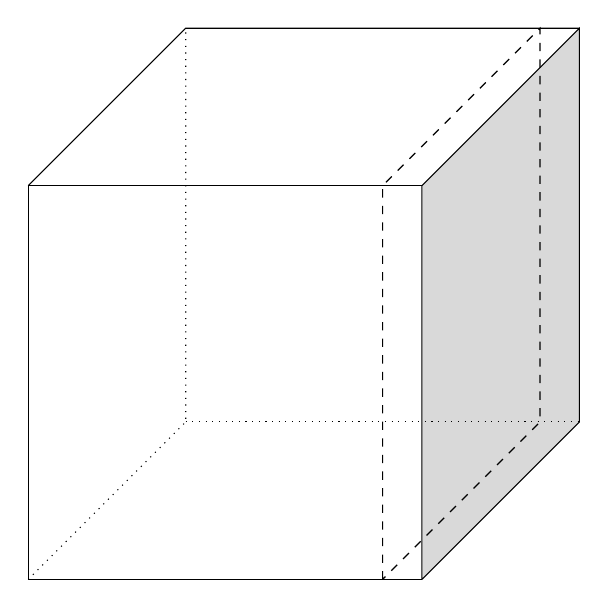
\begin{tikzpicture}
  \draw[fill=gray!30!white] (5,0)--(5,5)--(7,7)--(7,2)--(5,0);
  \draw (5,0)--(0,0)--(0,5)--(5,5);
  \draw (0,5)--(2,7)--(7,7);
  \draw[dotted] (0,0)--(2,2)--(2,7);
  \draw[dotted] (2,2)--(7,2);
  \draw[dashed] (4.5,0)--(4.5,5)--(6.5,7)--(6.5,2)--(4.5,0);
\end{tikzpicture}
\caption{Considerazioni cinetiche ed effusione di un gas. La parete di cui si parla nel testo è quella ombreggiata. Con una linea tratteggiata si è cercato di delineare l'elemento di volume $\de{V}$: le molecole che si trovano in questo volume e viaggiano verso destra colpiscono la parete in un tempo $\de{t}$. Naturalmente detto elemento di volume varia da molecola a molecola, e per questo quindi occorre integrare sulla distribuzione $f_v(v)$.}
\end{figure}
%%%%%%%%%%%%%%%%%%%%%%%%%%%%%%%%%%%%%%%%%%%%%%%%%%%%%%%%%%%%%%%%%%%%%%%%

Sia $A$ l'area della parete e $\hat x$ il versore in direzione $x$; consideriamo una particolare molecola con velocità $\myvec{v}$. Qualunque siano le componenti $y$ e $z$ della velocità, questa molecola colpirà la parete in questione nei prossimi $\de{t}$ secondi solo se è a una distanza inferiore o uguale a $\myvec{v}\cdot\hat x\,\de{t} = v_x\de{t}$ dalla parete. Per ottenere il numero totale di molecole che urtano la parete bisognerà dunque moltiplicare questa distanza per la densità $n = N/V$, per l'area $A$ della parete, per la distribuzione $f_v(v)$ e infine integrare su tutte le possibili velocità, tenendo presente che in $\de{v_x}$ occorre integrare solo da $0$ a $\infty$ (solo sulle molecole che si muovono in verso positivo). Chiamando $\de{N}$ il numero di molecole che colpiscono la parete in un tempo $\de{t}$ otteniamo:
\bea
\label{eq:pereff}
\de{N} &=& nA\de{t}\int_0^\infty\de{v_x} v_x f_{x}(v_x)\iint_{-\infty}^{\infty}\de{v_y}\de{v_z}f_{y}(v_y)f_{z}(v_z)\nonumber\\
&=& nA\sqrt{\dfrac{kT}{2\pi m}}
\eea
Ogni singolo urto trasferisce alla parete una certa quantità di moto; assumendo urti perfettamente elastici abbiamo che la quantità di moto trasferita in un singolo urto sarà pari alla variazione della quantità di moto della molecola presa con il segno negativo, cioè $2mv_x$. Per ottenere la quantità di moto totale trasferita in un tempo $\de{t}$ dobbiamo scrivere una formula identica alla (\ref{eq:pereff}), con $2mv_x^2$ al posto di $v_x$. Ma la derivata della quantità di moto rispetto al tempo è pari alla forza esercitata dal gas sulla parete, e dividendo per l'area otteniamo la pressione. Quindi
\bea
\label{eq:prescine}
P &=& 2mn\int_0^\infty\de{v_x} v_x^2 f_{x}(v_x)\iint_{-\infty}^{\infty}\de{v_y}\de{v_z}f_{y}(v_y)f_{z}(v_z)\nonumber\\
&=& \dfrac{NkT}{V}
\eea
Ritroviamo così la pressione di un gas ideale classico.

%%%%%%%%%%%%%%%%%%%%%%%%%%%%%%%%%%%%%%%%%%%%%%%%%%%%%%%%%%%%%%%%%%%%%%%%
\subsection{L'effusione di un gas}
\label{subsec:effusione}
%%%%%%%%%%%%%%%%%%%%%%%%%%%%%%%%%%%%%%%%%%%%%%%%%%%%%%%%%%%%%%%%%%%%%%%%

Se si pratica un piccolo foro di area $S$ sulla famosa parete, il gas fuoriesce dal contenitore effondendo nel vuoto. Assumiamo che il processo venga regolato in modo tale che la temperatura $T$ resti costante, almeno per un periodo di tempo finito (è noto che in generale l'effusione di un gas da un contenitore comporta il raffreddamento del gas che rimane dentro; pensate alle bombolette spray).

Per calcolare il {\em rate} di effusione, ossia il numero di molecole che fuoriescono dal contenitore per unità di tempo, è sufficiente considerare l'eq. (\ref{eq:pereff}) con l'area $S$ al posto dell'area $A$. Infatti le molecole che ``urtano'' il foro sono proprio quelle che escono. Otteniamo
%
\be
\frac{\de{N}}{\de{t}} = -nS\int_{0}^{\infty}\de{v_{x}} v_{x}f_{x}(v_{x})\int\int\limits_{0}^{\infty}\de{v_{y}}\de{v_{z}}f_{y}(v_{y})f_{z}(v_{z})
\ee
%
in cui il segno meno è dovuto al fatto che $N$ diminuisce in seguito all'effusione; in definitiva, confrontando con la (\ref{eq:vmediaMB}), abbiamo
%
\be
\frac{\de{N}}{\de{t}} = -\frac{nS}{4}\langle v \rangle
\ee
%
Poiché il gas è tenuto a temperatura costante $T$ abbiamo $PV = NkT$, e dall'equazione per $N$ otteniamo un'equazione per la pressione $P$:
%
\be
\frac{\de{P}}{P} = -\frac{\de{t}}{\tau_{0}}
\ee
%
in cui abbiamo introdotto la costante di tempo $\tau_{0} = \frac{4V}{S\langle v \rangle}$. Otteniamo quindi
%
\be
P(t) = P(0)e^{-t/\tau_{0}}
\ee
%

%%%%%%%%%%%%%%%%%%%%%%%%%%%%%%%%%%%%%%%%%%%%%%%%%%%%%%%%%%%%%%%%%%%%%%%%%
\section{Potenziale esterno: un esempio}
\label{sec:potesterno}
%%%%%%%%%%%%%%%%%%%%%%%%%%%%%%%%%%%%%%%%%%%%%%%%%%%%%%%%%%%%%%%%%%%%%%%%%

Notiamo subito una cosa: nonostante esista un potenziale esterno, il sistema è ancora non--interagente, nel senso che le particelle che lo compongono non interagiscono tra loro ma solo col potenziale esterno. Questo potenziale dovrà naturalmente soddisfare una serie di requisiti:
\begin{itemize}
\item dev'essere indipendente dal tempo;
\item deve variare lentamente sulla scala delle distanze tipiche tra le particelle e delle eventuali interazioni microscopiche;
\item non deve modificare in maniera sostanziale le eventuali interazioni intermolecolari (esempio: un forte campo elettrico applicato a molecole facilmente polarizzabili)
\end{itemize}

Consideriamo dunque come esempio un gas ideale classico racchiuso in un cilindro di area di base $S$ e altezza $L$. Il gas è sottoposto alla forza gravitazionale, considerata costante, e quindi a un potenziale lineare. Ci chiediamo quale sia la pressione esercitata dal gas sulla faccia superiore del cilindro.

Chiamando $y$ la coordinata verticale, per non confonderci con la fugacità, abbiamo che l'Hamiltoniana di singola particella è
%
\be
\Ham = \frac{1}{2m}p^{2} + mgy
\ee
%
in cui $g$ è l'accelerazione di gravità. La funzione di partizione di singola particella può essere scritta come
%
\be
Q_{1} = \frac{1}{h^{3}}\int\de{p}\,(4\pi p^{2})e^{-\beta p^{2}/2m}\int_{S}\de{x}\,\de{z}
\int_{0}^{L}\de{y}\,e^{-\beta mgy}
\ee
%
e un semplice calcolo ci fornisce
%
\be
Q_{1} = \frac{2\pi S}{gh^{3}}\frac{(2\pi m)^{1/2}}{\beta^{5/2}}(1-e^{-\beta mgL})
\ee
%
Dalla funzione di partizione otteniamo subito l'energia libera di Helmholtz:
%
\be
A = -kT\ln Q_{N} = -NkT(\ln Q_{1} - \ln N + 1)
\ee
%
in cui abbiamo usato la formula di Stirling per calcolare il $\ln(N!)$. In generale derivando $A$ rispetto a $V$ si ottiene la pressione sulle pareti del contenitore, ma questa volta non possiamo derivare direttamente in questo modo perché la forza di gravità fa sì che la densità delle molecole, e dunque la pressione, non sia costante ma vari con l'altezza.

Però se vogliamo sapere la pressione sulla faccia superiore del cilindro possiamo scrivere $V = SL$ e derivare rispetto a $L$:
%
\be
\label{eq:PaL}
P(L) = -\frac{1}{S}\dpar{A}{L} = \frac{Nmg}{S}\frac{e^{-\beta mgL}}{1-e^{-\beta mgL}}
\ee
%

Se invece vogliamo sapere come varia la pressione in funzione dell'altezza dobbiamo seguire un'altra strada.
Notiamo che in condizioni di equilibrio, pur se sottoposto a un generico potenziale esterno, $U(\myvec{r})$, nel gas non possono avvenire spostamenti netti di materia. Ciò significa che il potenziale chimico deve essere costante, e in particolare non deve dipendere da $y$. Riprenderemo questo discorso nella sezione \ref{sec:potesternoGC} del capitolo \ref{cap:grancanonico}, dopo che avremo sviluppato il formalismo dell'ensemble grancanonico.

%%%%%%%%%%%%%%%%%%%%%%%%%%%%%%%%%%%%%%%%%%%%%%%%%%%%%%%%%%%%%%%%%%%%%%%%%
\section{Esercizi per il capitolo \ref{cap:canonico}}
%%%%%%%%%%%%%%%%%%%%%%%%%%%%%%%%%%%%%%%%%%%%%%%%%%%%%%%%%%%%%%%%%%%%%%%%%

%-----------------------------------------------------------------------
% GAS ULTRARELATIVISTICO
%-----------------------------------------------------------------------
\begin{Exercise}[title={Ancora sul gas ideale classico ultrarelativistico},
label={ex:04-guc}]
Si ripeta l'esercizio \ref{ex:03-gicur} utilizzando il formalismo canonico. Inoltre si calcoli la densità degli stati partendo dalla funzione di partizione. Si confronti il risultato con il numero degli stati ottenuto col formalismo microcanonico.
\end{Exercise}

%-----------------------------------------------------------------------
% OSCILLATORI DI FERMI
%-----------------------------------------------------------------------
\begin{Exercise}[title={Oscillatori di Fermi, la vendetta canonica},
label={ex:04-oscfermi}]
Riconsiderare l'esercizio \ref{ex:03-oscfermi} alla luce del formalismo canonico.
\end{Exercise}

%-----------------------------------------------------------------------
% EQUILIBRIO CHIMICO
%-----------------------------------------------------------------------
\begin{Exercise}[title={Equilibrio chimico},label={ex:04-eqchim}]
Si consideri un gas ideale classico composto da atomi di tipo $a$, atomi di tipo $b$ e molecole $ab$. Il sistema è racchiuso in un volume $V$ e le reazioni
\be
a + b \rightleftharpoons ab
\ee
avvengono all'equilibrio a una temperatura $T$. Chiamando $n_x$ le densità ($n_x = N_x/V$) e $Q_x$ le funzioni di partizione di singola particella, si dimostri che vale la relazione
\be
\frac{n_{ab}}{n_a n_b} = V\frac{Q_{ab}}{Q_a Q_b}
\ee
\end{Exercise}

%-----------------------------------------------------------------------
% ENTROPIA GAS IDEALE CLASSICO
%-----------------------------------------------------------------------
\begin{Exercise}[title={Entropia di un gas ideale classico},label={ex:04-esps}]
Mostrare che per un gas ideale classico vale la relazione
\be
\frac{S}{Nk} = \ln\left(\frac{Q_1}{N}\right) + T\dparc{\ln Q_1}{T}{P}
\ee
in cui $Q_1$ è la funzione di partizione canonica di singola particella.
\end{Exercise}

%%%%%%%%%%%%%%%%%%%%%%%%%%%%%%%%%%%%%%%%%%%%%%%%%%%%%%%%%%%%%%%%%%%%%%

\vskip 0.75cm
\begin{flushright}
{\em Ultimo aggiornamento del capitolo: 21.04.2017}
\end{flushright}

